\documentclass[a4paper, 12pt]{article}
\usepackage[left=2cm,right=2cm, top=2cm,bottom=2cm,bindingoffset=0cm]{geometry}
\usepackage{cmap, amssymb, amsmath, amsthm, mathtools}
\usepackage{upgreek}
\usepackage{setspace}
\usepackage{mathtext}

    \usepackage[breakable]{tcolorbox}
    \usepackage{parskip} % Stop auto-indenting (to mimic markdown behaviour)
    

    % Basic figure setup, for now with no caption control since it's done
    % automatically by Pandoc (which extracts ![](path) syntax from Markdown).
    \usepackage{graphicx}
    % Keep aspect ratio if custom image width or height is specified
    \setkeys{Gin}{keepaspectratio}
    % Maintain compatibility with old templates. Remove in nbconvert 6.0
    \let\Oldincludegraphics\includegraphics
    % Ensure that by default, figures have no caption (until we provide a
    % proper Figure object with a Caption API and a way to capture that
    % in the conversion process - todo).
    \usepackage{caption}
    \DeclareCaptionFormat{nocaption}{}
    \captionsetup{format=nocaption,aboveskip=0pt,belowskip=0pt}

    \usepackage{float}
    \floatplacement{figure}{H} % forces figures to be placed at the correct location
    \usepackage{xcolor} % Allow colors to be defined
    \usepackage{enumerate} % Needed for markdown enumerations to work
    \usepackage{geometry} % Used to adjust the document margins
    \usepackage{amsmath} % Equations
    \usepackage{amssymb} % Equations
    \usepackage{textcomp} % defines textquotesingle
    % Hack from http://tex.stackexchange.com/a/47451/13684:
    \AtBeginDocument{%
        \def\PYZsq{\textquotesingle}% Upright quotes in Pygmentized code
    }
    \usepackage{upquote} % Upright quotes for verbatim code
    \usepackage{eurosym} % defines \euro

    \usepackage{iftex}
    \ifPDFTeX
        \usepackage[T2A]{fontenc}
        \IfFileExists{alphabeta.sty}{
              \usepackage{alphabeta}
          }{
              \usepackage[mathletters]{ucs}
              \usepackage[utf8]{inputenc}
          }
    \else
        \usepackage{fontspec}
        \usepackage{unicode-math}
    \fi

    \usepackage{fancyvrb} % verbatim replacement that allows latex
    \usepackage{grffile} % extends the file name processing of package graphics
                         % to support a larger range
    \makeatletter % fix for old versions of grffile with XeLaTeX
    \@ifpackagelater{grffile}{2019/11/01}
    {
      % Do nothing on new versions
    }
    {
      \def\Gread@@xetex#1{%
        \IfFileExists{"\Gin@base".bb}%
        {\Gread@eps{\Gin@base.bb}}%
        {\Gread@@xetex@aux#1}%
      }
    }
    \makeatother
    \usepackage[Export]{adjustbox} % Used to constrain images to a maximum size
    \adjustboxset{max size={0.9\linewidth}{0.9\paperheight}}

    % The hyperref package gives us a pdf with properly built
    % internal navigation ('pdf bookmarks' for the table of contents,
    % internal cross-reference links, web links for URLs, etc.)
    \usepackage{hyperref}
    % The default LaTeX title has an obnoxious amount of whitespace. By default,
    % titling removes some of it. It also provides customization options.
    \usepackage{titling}
    \usepackage{longtable} % longtable support required by pandoc >1.10
    \usepackage{booktabs}  % table support for pandoc > 1.12.2
    \usepackage{array}     % table support for pandoc >= 2.11.3
    \usepackage{calc}      % table minipage width calculation for pandoc >= 2.11.1
    \usepackage[inline]{enumitem} % IRkernel/repr support (it uses the enumerate* environment)
    \usepackage[normalem]{ulem} % ulem is needed to support strikethroughs (\sout)
                                % normalem makes italics be italics, not underlines
    \usepackage{soul}      % strikethrough (\st) support for pandoc >= 3.0.0
    \usepackage{mathrsfs}
    

    
    % Colors for the hyperref package
    \definecolor{urlcolor}{rgb}{0,.145,.698}
    \definecolor{linkcolor}{rgb}{.71,0.21,0.01}
    \definecolor{citecolor}{rgb}{.12,.54,.11}

    % ANSI colors
    \definecolor{ansi-black}{HTML}{3E424D}
    \definecolor{ansi-black-intense}{HTML}{282C36}
    \definecolor{ansi-red}{HTML}{E75C58}
    \definecolor{ansi-red-intense}{HTML}{B22B31}
    \definecolor{ansi-green}{HTML}{00A250}
    \definecolor{ansi-green-intense}{HTML}{007427}
    \definecolor{ansi-yellow}{HTML}{DDB62B}
    \definecolor{ansi-yellow-intense}{HTML}{B27D12}
    \definecolor{ansi-blue}{HTML}{208FFB}
    \definecolor{ansi-blue-intense}{HTML}{0065CA}
    \definecolor{ansi-magenta}{HTML}{D160C4}
    \definecolor{ansi-magenta-intense}{HTML}{A03196}
    \definecolor{ansi-cyan}{HTML}{60C6C8}
    \definecolor{ansi-cyan-intense}{HTML}{258F8F}
    \definecolor{ansi-white}{HTML}{C5C1B4}
    \definecolor{ansi-white-intense}{HTML}{A1A6B2}
    \definecolor{ansi-default-inverse-fg}{HTML}{FFFFFF}
    \definecolor{ansi-default-inverse-bg}{HTML}{000000}

    % common color for the border for error outputs.
    \definecolor{outerrorbackground}{HTML}{FFDFDF}

    % commands and environments needed by pandoc snippets
    % extracted from the output of `pandoc -s`
    \providecommand{\tightlist}{%
      \setlength{\itemsep}{0pt}\setlength{\parskip}{0pt}}
    \DefineVerbatimEnvironment{Highlighting}{Verbatim}{commandchars=\\\{\}}
    % Add ',fontsize=\small' for more characters per line
    \newenvironment{Shaded}{}{}
    \newcommand{\KeywordTok}[1]{\textcolor[rgb]{0.00,0.44,0.13}{\textbf{{#1}}}}
    \newcommand{\DataTypeTok}[1]{\textcolor[rgb]{0.56,0.13,0.00}{{#1}}}
    \newcommand{\DecValTok}[1]{\textcolor[rgb]{0.25,0.63,0.44}{{#1}}}
    \newcommand{\BaseNTok}[1]{\textcolor[rgb]{0.25,0.63,0.44}{{#1}}}
    \newcommand{\FloatTok}[1]{\textcolor[rgb]{0.25,0.63,0.44}{{#1}}}
    \newcommand{\CharTok}[1]{\textcolor[rgb]{0.25,0.44,0.63}{{#1}}}
    \newcommand{\StringTok}[1]{\textcolor[rgb]{0.25,0.44,0.63}{{#1}}}
    \newcommand{\CommentTok}[1]{\textcolor[rgb]{0.38,0.63,0.69}{\textit{{#1}}}}
    \newcommand{\OtherTok}[1]{\textcolor[rgb]{0.00,0.44,0.13}{{#1}}}
    \newcommand{\AlertTok}[1]{\textcolor[rgb]{1.00,0.00,0.00}{\textbf{{#1}}}}
    \newcommand{\FunctionTok}[1]{\textcolor[rgb]{0.02,0.16,0.49}{{#1}}}
    \newcommand{\RegionMarkerTok}[1]{{#1}}
    \newcommand{\ErrorTok}[1]{\textcolor[rgb]{1.00,0.00,0.00}{\textbf{{#1}}}}
    \newcommand{\NormalTok}[1]{{#1}}

    % Additional commands for more recent versions of Pandoc
    \newcommand{\ConstantTok}[1]{\textcolor[rgb]{0.53,0.00,0.00}{{#1}}}
    \newcommand{\SpecialCharTok}[1]{\textcolor[rgb]{0.25,0.44,0.63}{{#1}}}
    \newcommand{\VerbatimStringTok}[1]{\textcolor[rgb]{0.25,0.44,0.63}{{#1}}}
    \newcommand{\SpecialStringTok}[1]{\textcolor[rgb]{0.73,0.40,0.53}{{#1}}}
    \newcommand{\ImportTok}[1]{{#1}}
    \newcommand{\DocumentationTok}[1]{\textcolor[rgb]{0.73,0.13,0.13}{\textit{{#1}}}}
    \newcommand{\AnnotationTok}[1]{\textcolor[rgb]{0.38,0.63,0.69}{\textbf{\textit{{#1}}}}}
    \newcommand{\CommentVarTok}[1]{\textcolor[rgb]{0.38,0.63,0.69}{\textbf{\textit{{#1}}}}}
    \newcommand{\VariableTok}[1]{\textcolor[rgb]{0.10,0.09,0.49}{{#1}}}
    \newcommand{\ControlFlowTok}[1]{\textcolor[rgb]{0.00,0.44,0.13}{\textbf{{#1}}}}
    \newcommand{\OperatorTok}[1]{\textcolor[rgb]{0.40,0.40,0.40}{{#1}}}
    \newcommand{\BuiltInTok}[1]{{#1}}
    \newcommand{\ExtensionTok}[1]{{#1}}
    \newcommand{\PreprocessorTok}[1]{\textcolor[rgb]{0.74,0.48,0.00}{{#1}}}
    \newcommand{\AttributeTok}[1]{\textcolor[rgb]{0.49,0.56,0.16}{{#1}}}
    \newcommand{\InformationTok}[1]{\textcolor[rgb]{0.38,0.63,0.69}{\textbf{\textit{{#1}}}}}
    \newcommand{\WarningTok}[1]{\textcolor[rgb]{0.38,0.63,0.69}{\textbf{\textit{{#1}}}}}


    % Define a nice break command that doesn't care if a line doesn't already
    % exist.
    \def\br{\hspace*{\fill} \\* }
    % Math Jax compatibility definitions
    \def\gt{>}
    \def\lt{<}
    \let\Oldtex\TeX
    \let\Oldlatex\LaTeX
    \renewcommand{\TeX}{\textrm{\Oldtex}}
    \renewcommand{\LaTeX}{\textrm{\Oldlatex}}
    % Document parameters
    % Document title
    \title{notebook}
    
    
    
    
    
    
    
% Pygments definitions
\makeatletter
\def\PY@reset{\let\PY@it=\relax \let\PY@bf=\relax%
    \let\PY@ul=\relax \let\PY@tc=\relax%
    \let\PY@bc=\relax \let\PY@ff=\relax}
\def\PY@tok#1{\csname PY@tok@#1\endcsname}
\def\PY@toks#1+{\ifx\relax#1\empty\else%
    \PY@tok{#1}\expandafter\PY@toks\fi}
\def\PY@do#1{\PY@bc{\PY@tc{\PY@ul{%
    \PY@it{\PY@bf{\PY@ff{#1}}}}}}}
\def\PY#1#2{\PY@reset\PY@toks#1+\relax+\PY@do{#2}}

\@namedef{PY@tok@w}{\def\PY@tc##1{\textcolor[rgb]{0.73,0.73,0.73}{##1}}}
\@namedef{PY@tok@c}{\let\PY@it=\textit\def\PY@tc##1{\textcolor[rgb]{0.24,0.48,0.48}{##1}}}
\@namedef{PY@tok@cp}{\def\PY@tc##1{\textcolor[rgb]{0.61,0.40,0.00}{##1}}}
\@namedef{PY@tok@k}{\let\PY@bf=\textbf\def\PY@tc##1{\textcolor[rgb]{0.00,0.50,0.00}{##1}}}
\@namedef{PY@tok@kp}{\def\PY@tc##1{\textcolor[rgb]{0.00,0.50,0.00}{##1}}}
\@namedef{PY@tok@kt}{\def\PY@tc##1{\textcolor[rgb]{0.69,0.00,0.25}{##1}}}
\@namedef{PY@tok@o}{\def\PY@tc##1{\textcolor[rgb]{0.40,0.40,0.40}{##1}}}
\@namedef{PY@tok@ow}{\let\PY@bf=\textbf\def\PY@tc##1{\textcolor[rgb]{0.67,0.13,1.00}{##1}}}
\@namedef{PY@tok@nb}{\def\PY@tc##1{\textcolor[rgb]{0.00,0.50,0.00}{##1}}}
\@namedef{PY@tok@nf}{\def\PY@tc##1{\textcolor[rgb]{0.00,0.00,1.00}{##1}}}
\@namedef{PY@tok@nc}{\let\PY@bf=\textbf\def\PY@tc##1{\textcolor[rgb]{0.00,0.00,1.00}{##1}}}
\@namedef{PY@tok@nn}{\let\PY@bf=\textbf\def\PY@tc##1{\textcolor[rgb]{0.00,0.00,1.00}{##1}}}
\@namedef{PY@tok@ne}{\let\PY@bf=\textbf\def\PY@tc##1{\textcolor[rgb]{0.80,0.25,0.22}{##1}}}
\@namedef{PY@tok@nv}{\def\PY@tc##1{\textcolor[rgb]{0.10,0.09,0.49}{##1}}}
\@namedef{PY@tok@no}{\def\PY@tc##1{\textcolor[rgb]{0.53,0.00,0.00}{##1}}}
\@namedef{PY@tok@nl}{\def\PY@tc##1{\textcolor[rgb]{0.46,0.46,0.00}{##1}}}
\@namedef{PY@tok@ni}{\let\PY@bf=\textbf\def\PY@tc##1{\textcolor[rgb]{0.44,0.44,0.44}{##1}}}
\@namedef{PY@tok@na}{\def\PY@tc##1{\textcolor[rgb]{0.41,0.47,0.13}{##1}}}
\@namedef{PY@tok@nt}{\let\PY@bf=\textbf\def\PY@tc##1{\textcolor[rgb]{0.00,0.50,0.00}{##1}}}
\@namedef{PY@tok@nd}{\def\PY@tc##1{\textcolor[rgb]{0.67,0.13,1.00}{##1}}}
\@namedef{PY@tok@s}{\def\PY@tc##1{\textcolor[rgb]{0.73,0.13,0.13}{##1}}}
\@namedef{PY@tok@sd}{\let\PY@it=\textit\def\PY@tc##1{\textcolor[rgb]{0.73,0.13,0.13}{##1}}}
\@namedef{PY@tok@si}{\let\PY@bf=\textbf\def\PY@tc##1{\textcolor[rgb]{0.64,0.35,0.47}{##1}}}
\@namedef{PY@tok@se}{\let\PY@bf=\textbf\def\PY@tc##1{\textcolor[rgb]{0.67,0.36,0.12}{##1}}}
\@namedef{PY@tok@sr}{\def\PY@tc##1{\textcolor[rgb]{0.64,0.35,0.47}{##1}}}
\@namedef{PY@tok@ss}{\def\PY@tc##1{\textcolor[rgb]{0.10,0.09,0.49}{##1}}}
\@namedef{PY@tok@sx}{\def\PY@tc##1{\textcolor[rgb]{0.00,0.50,0.00}{##1}}}
\@namedef{PY@tok@m}{\def\PY@tc##1{\textcolor[rgb]{0.40,0.40,0.40}{##1}}}
\@namedef{PY@tok@gh}{\let\PY@bf=\textbf\def\PY@tc##1{\textcolor[rgb]{0.00,0.00,0.50}{##1}}}
\@namedef{PY@tok@gu}{\let\PY@bf=\textbf\def\PY@tc##1{\textcolor[rgb]{0.50,0.00,0.50}{##1}}}
\@namedef{PY@tok@gd}{\def\PY@tc##1{\textcolor[rgb]{0.63,0.00,0.00}{##1}}}
\@namedef{PY@tok@gi}{\def\PY@tc##1{\textcolor[rgb]{0.00,0.52,0.00}{##1}}}
\@namedef{PY@tok@gr}{\def\PY@tc##1{\textcolor[rgb]{0.89,0.00,0.00}{##1}}}
\@namedef{PY@tok@ge}{\let\PY@it=\textit}
\@namedef{PY@tok@gs}{\let\PY@bf=\textbf}
\@namedef{PY@tok@ges}{\let\PY@bf=\textbf\let\PY@it=\textit}
\@namedef{PY@tok@gp}{\let\PY@bf=\textbf\def\PY@tc##1{\textcolor[rgb]{0.00,0.00,0.50}{##1}}}
\@namedef{PY@tok@go}{\def\PY@tc##1{\textcolor[rgb]{0.44,0.44,0.44}{##1}}}
\@namedef{PY@tok@gt}{\def\PY@tc##1{\textcolor[rgb]{0.00,0.27,0.87}{##1}}}
\@namedef{PY@tok@err}{\def\PY@bc##1{{\setlength{\fboxsep}{\string -\fboxrule}\fcolorbox[rgb]{1.00,0.00,0.00}{1,1,1}{\strut ##1}}}}
\@namedef{PY@tok@kc}{\let\PY@bf=\textbf\def\PY@tc##1{\textcolor[rgb]{0.00,0.50,0.00}{##1}}}
\@namedef{PY@tok@kd}{\let\PY@bf=\textbf\def\PY@tc##1{\textcolor[rgb]{0.00,0.50,0.00}{##1}}}
\@namedef{PY@tok@kn}{\let\PY@bf=\textbf\def\PY@tc##1{\textcolor[rgb]{0.00,0.50,0.00}{##1}}}
\@namedef{PY@tok@kr}{\let\PY@bf=\textbf\def\PY@tc##1{\textcolor[rgb]{0.00,0.50,0.00}{##1}}}
\@namedef{PY@tok@bp}{\def\PY@tc##1{\textcolor[rgb]{0.00,0.50,0.00}{##1}}}
\@namedef{PY@tok@fm}{\def\PY@tc##1{\textcolor[rgb]{0.00,0.00,1.00}{##1}}}
\@namedef{PY@tok@vc}{\def\PY@tc##1{\textcolor[rgb]{0.10,0.09,0.49}{##1}}}
\@namedef{PY@tok@vg}{\def\PY@tc##1{\textcolor[rgb]{0.10,0.09,0.49}{##1}}}
\@namedef{PY@tok@vi}{\def\PY@tc##1{\textcolor[rgb]{0.10,0.09,0.49}{##1}}}
\@namedef{PY@tok@vm}{\def\PY@tc##1{\textcolor[rgb]{0.10,0.09,0.49}{##1}}}
\@namedef{PY@tok@sa}{\def\PY@tc##1{\textcolor[rgb]{0.73,0.13,0.13}{##1}}}
\@namedef{PY@tok@sb}{\def\PY@tc##1{\textcolor[rgb]{0.73,0.13,0.13}{##1}}}
\@namedef{PY@tok@sc}{\def\PY@tc##1{\textcolor[rgb]{0.73,0.13,0.13}{##1}}}
\@namedef{PY@tok@dl}{\def\PY@tc##1{\textcolor[rgb]{0.73,0.13,0.13}{##1}}}
\@namedef{PY@tok@s2}{\def\PY@tc##1{\textcolor[rgb]{0.73,0.13,0.13}{##1}}}
\@namedef{PY@tok@sh}{\def\PY@tc##1{\textcolor[rgb]{0.73,0.13,0.13}{##1}}}
\@namedef{PY@tok@s1}{\def\PY@tc##1{\textcolor[rgb]{0.73,0.13,0.13}{##1}}}
\@namedef{PY@tok@mb}{\def\PY@tc##1{\textcolor[rgb]{0.40,0.40,0.40}{##1}}}
\@namedef{PY@tok@mf}{\def\PY@tc##1{\textcolor[rgb]{0.40,0.40,0.40}{##1}}}
\@namedef{PY@tok@mh}{\def\PY@tc##1{\textcolor[rgb]{0.40,0.40,0.40}{##1}}}
\@namedef{PY@tok@mi}{\def\PY@tc##1{\textcolor[rgb]{0.40,0.40,0.40}{##1}}}
\@namedef{PY@tok@il}{\def\PY@tc##1{\textcolor[rgb]{0.40,0.40,0.40}{##1}}}
\@namedef{PY@tok@mo}{\def\PY@tc##1{\textcolor[rgb]{0.40,0.40,0.40}{##1}}}
\@namedef{PY@tok@ch}{\let\PY@it=\textit\def\PY@tc##1{\textcolor[rgb]{0.24,0.48,0.48}{##1}}}
\@namedef{PY@tok@cm}{\let\PY@it=\textit\def\PY@tc##1{\textcolor[rgb]{0.24,0.48,0.48}{##1}}}
\@namedef{PY@tok@cpf}{\let\PY@it=\textit\def\PY@tc##1{\textcolor[rgb]{0.24,0.48,0.48}{##1}}}
\@namedef{PY@tok@c1}{\let\PY@it=\textit\def\PY@tc##1{\textcolor[rgb]{0.24,0.48,0.48}{##1}}}
\@namedef{PY@tok@cs}{\let\PY@it=\textit\def\PY@tc##1{\textcolor[rgb]{0.24,0.48,0.48}{##1}}}

\def\PYZbs{\char`\\}
\def\PYZus{\char`\_}
\def\PYZob{\char`\{}
\def\PYZcb{\char`\}}
\def\PYZca{\char`\^}
\def\PYZam{\char`\&}
\def\PYZlt{\char`\<}
\def\PYZgt{\char`\>}
\def\PYZsh{\char`\#}
\def\PYZpc{\char`\%}
\def\PYZdl{\char`\$}
\def\PYZhy{\char`\-}
\def\PYZsq{\char`\'}
\def\PYZdq{\char`\"}
\def\PYZti{\char`\~}
% for compatibility with earlier versions
\def\PYZat{@}
\def\PYZlb{[}
\def\PYZrb{]}
\makeatother


    % For linebreaks inside Verbatim environment from package fancyvrb.
    \makeatletter
        \newbox\Wrappedcontinuationbox
        \newbox\Wrappedvisiblespacebox
        \newcommand*\Wrappedvisiblespace {\textcolor{red}{\textvisiblespace}}
        \newcommand*\Wrappedcontinuationsymbol {\textcolor{red}{\llap{\tiny$\m@th\hookrightarrow$}}}
        \newcommand*\Wrappedcontinuationindent {3ex }
        \newcommand*\Wrappedafterbreak {\kern\Wrappedcontinuationindent\copy\Wrappedcontinuationbox}
        % Take advantage of the already applied Pygments mark-up to insert
        % potential linebreaks for TeX processing.
        %        {, <, #, %, $, ' and ": go to next line.
        %        _, }, ^, &, >, - and ~: stay at end of broken line.
        % Use of \textquotesingle for straight quote.
        \newcommand*\Wrappedbreaksatspecials {%
            \def\PYGZus{\discretionary{\char`\_}{\Wrappedafterbreak}{\char`\_}}%
            \def\PYGZob{\discretionary{}{\Wrappedafterbreak\char`\{}{\char`\{}}%
            \def\PYGZcb{\discretionary{\char`\}}{\Wrappedafterbreak}{\char`\}}}%
            \def\PYGZca{\discretionary{\char`\^}{\Wrappedafterbreak}{\char`\^}}%
            \def\PYGZam{\discretionary{\char`\&}{\Wrappedafterbreak}{\char`\&}}%
            \def\PYGZlt{\discretionary{}{\Wrappedafterbreak\char`\<}{\char`\<}}%
            \def\PYGZgt{\discretionary{\char`\>}{\Wrappedafterbreak}{\char`\>}}%
            \def\PYGZsh{\discretionary{}{\Wrappedafterbreak\char`\#}{\char`\#}}%
            \def\PYGZpc{\discretionary{}{\Wrappedafterbreak\char`\%}{\char`\%}}%
            \def\PYGZdl{\discretionary{}{\Wrappedafterbreak\char`\$}{\char`\$}}%
            \def\PYGZhy{\discretionary{\char`\-}{\Wrappedafterbreak}{\char`\-}}%
            \def\PYGZsq{\discretionary{}{\Wrappedafterbreak\textquotesingle}{\textquotesingle}}%
            \def\PYGZdq{\discretionary{}{\Wrappedafterbreak\char`\"}{\char`\"}}%
            \def\PYGZti{\discretionary{\char`\~}{\Wrappedafterbreak}{\char`\~}}%
        }
        % Some characters . , ; ? ! / are not pygmentized.
        % This macro makes them "active" and they will insert potential linebreaks
        \newcommand*\Wrappedbreaksatpunct {%
            \lccode`\~`\.\lowercase{\def~}{\discretionary{\hbox{\char`\.}}{\Wrappedafterbreak}{\hbox{\char`\.}}}%
            \lccode`\~`\,\lowercase{\def~}{\discretionary{\hbox{\char`\,}}{\Wrappedafterbreak}{\hbox{\char`\,}}}%
            \lccode`\~`\;\lowercase{\def~}{\discretionary{\hbox{\char`\;}}{\Wrappedafterbreak}{\hbox{\char`\;}}}%
            \lccode`\~`\:\lowercase{\def~}{\discretionary{\hbox{\char`\:}}{\Wrappedafterbreak}{\hbox{\char`\:}}}%
            \lccode`\~`\?\lowercase{\def~}{\discretionary{\hbox{\char`\?}}{\Wrappedafterbreak}{\hbox{\char`\?}}}%
            \lccode`\~`\!\lowercase{\def~}{\discretionary{\hbox{\char`\!}}{\Wrappedafterbreak}{\hbox{\char`\!}}}%
            \lccode`\~`\/\lowercase{\def~}{\discretionary{\hbox{\char`\/}}{\Wrappedafterbreak}{\hbox{\char`\/}}}%
            \catcode`\.\active
            \catcode`\,\active
            \catcode`\;\active
            \catcode`\:\active
            \catcode`\?\active
            \catcode`\!\active
            \catcode`\/\active
            \lccode`\~`\~
        }
    \makeatother

    \let\OriginalVerbatim=\Verbatim
    \makeatletter
    \renewcommand{\Verbatim}[1][1]{%
        %\parskip\z@skip
        \sbox\Wrappedcontinuationbox {\Wrappedcontinuationsymbol}%
        \sbox\Wrappedvisiblespacebox {\FV@SetupFont\Wrappedvisiblespace}%
        \def\FancyVerbFormatLine ##1{\hsize\linewidth
            \vtop{\raggedright\hyphenpenalty\z@\exhyphenpenalty\z@
                \doublehyphendemerits\z@\finalhyphendemerits\z@
                \strut ##1\strut}%
        }%
        % If the linebreak is at a space, the latter will be displayed as visible
        % space at end of first line, and a continuation symbol starts next line.
        % Stretch/shrink are however usually zero for typewriter font.
        \def\FV@Space {%
            \nobreak\hskip\z@ plus\fontdimen3\font minus\fontdimen4\font
            \discretionary{\copy\Wrappedvisiblespacebox}{\Wrappedafterbreak}
            {\kern\fontdimen2\font}%
        }%

        % Allow breaks at special characters using \PYG... macros.
        \Wrappedbreaksatspecials
        % Breaks at punctuation characters . , ; ? ! and / need catcode=\active
        \OriginalVerbatim[#1,codes*=\Wrappedbreaksatpunct]%
    }
    \makeatother

    % Exact colors from NB
    \definecolor{incolor}{HTML}{303F9F}
    \definecolor{outcolor}{HTML}{D84315}
    \definecolor{cellborder}{HTML}{CFCFCF}
    \definecolor{cellbackground}{HTML}{F7F7F7}

    % prompt
    \makeatletter
    \newcommand{\boxspacing}{\kern\kvtcb@left@rule\kern\kvtcb@boxsep}
    \makeatother
    \newcommand{\prompt}[4]{
        {\ttfamily\llap{{\color{#2}[#3]:\hspace{3pt}#4}}\vspace{-\baselineskip}}
    }
    

    
    % Prevent overflowing lines due to hard-to-break entities
    \sloppy
    % Setup hyperref package
    \hypersetup{
      breaklinks=true,  % so long urls are correctly broken across lines
      colorlinks=true,
      urlcolor=urlcolor,
      linkcolor=linkcolor,
      citecolor=citecolor,
      }
    % Slightly bigger margins than the latex defaults
    
    \renewcommand{\d}{\partial}
    \newcommand\Norm[1]{\left\| #1 \right\|}

\begin{document}
    
    	% Оформление титульного листа
    	\begin{titlepage}
    		\begin{center}
    			\textsc{МИНИСТЕРСТВО ОБРАЗОВАНИЯ РЕСПУБЛИКИ БЕЛАРУСЬ БЕЛОРУССКИЙ ГОСУДАРСТВЕННЫЙ УНИВЕРСИТЕТ
    				\\[5mm]
    				Факультет прикладной математики и информатики\\[2mm]
    				Кафедра вычислительной математики
    			}
    			
    			\vfill
    			
    			\textbf{Лабораторная работа №4
    				\\[3mm]
    				«Разностная схема для уравнения теплопроводности»\\[6mm]
    				Вариант 4
    				\\[20mm]
    			}
    		\end{center}
    		
    		\hfill
    		\begin{minipage}{.4\textwidth}
    			Выполнила:\\[2mm] 
    			Гут Валерия Александровна\\
    			студентка 4 курса 7 группы\\[5mm]
    			
    			Преподаватель:\\[2mm] 
    			Репников Василий Иванович
    		\end{minipage}%
    		\vfill
    		\begin{center}
    			Минск, 2024\ г.
    		\end{center}
    	\end{titlepage}
    	
    	\newpage
    	\section*{Постановка задачи 1}
    	Поставлена третья краевая задача для уравнения теплопроводности с постоянными коэффициентами
    	\begin{equation}
    		\begin{cases}
    			\dfrac{\d u}{\d t} = \dfrac{\d ^2 u}{\d x^2} + \sqrt 2\sin \left(\dfrac \pi 4  + x + t\right),\ t>0,\ 0 < x < 1,\\
    			u(x,0) = \sin x,\ 0 \leq x \leq 1,\\
    			\dfrac{\d u(0,t)}{\d x} - 2u(0, t) = \cos t - 2 \sin t,\ t\geq 0\\ 
    			u(1,t) = \sin(t+1),\ t\geq 0.
    		\end{cases}
    	\end{equation}
    	\section*{Построение разностной схемы}
    	Сперва проверим корректную постановку данной дифференциальной задачи, для чего рассмотрим условия согласования:
    	$$\dfrac{\d \sin x}{\d x} - 2\sin x|_{x=0} = 1 = \cos t - 2\sin t|_{t = 0},$$
    	$$\cos x|_{x=1} = \sin 1 = \sin(t+1)|_{t=0}.$$
    	Таким образом, условия согласования выполнены. Также для данной задачи выполняется принцип максимума, который позволяет заключить, что если решение задачи существует, то оно единственно. Следовательно, дифференциальная задача является корректно поставленной.\\\\
    	Поставленная дифференциальная задача имеет точное решение $$u(x,t) = \sin(x+t).$$
    	Зададим равномерную по каждому направлению сетку
    	$$\overline\omega_{h\tau} = \overline \omega_h \times \overline \omega_\tau,\ \overline \omega_h = \{x_k = kh,\ k = \overline{0,N},\ Nh = 1\}, \ \overline \omega_\tau = \{t_j = j\tau,\ j=\overline{0,N_1},\ N_1\tau=T\}.$$
    	На этой сетке зададим шеститочечный шаблон
    	$$
    	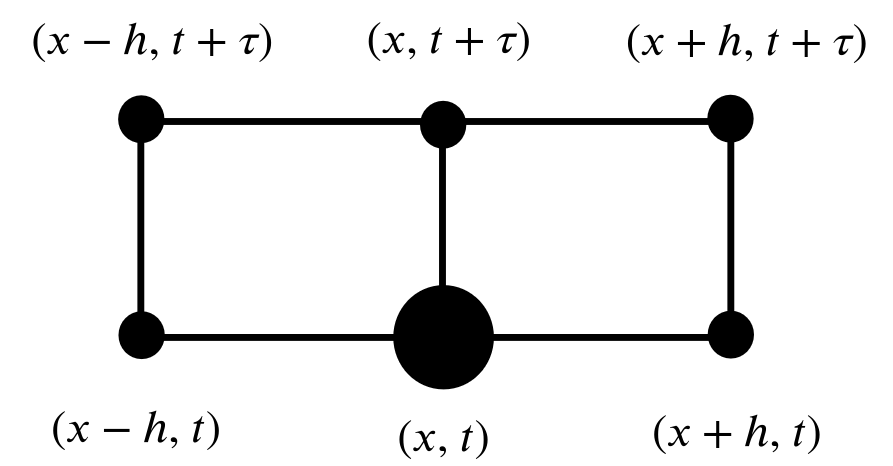
\includegraphics[scale=0.4]{images/img_5}
    	$$
    	Используя данный шаблон и заменяя дифференциальные операторы разностными, можем записать разностную схему для поставленной задачи в бензиндексной форме
    	\begin{equation}
    		\begin{cases}
    			y_t = \Lambda(\sigma \hat y + (1-\sigma)y)+\varphi,\ (x,t)\in \omega_{h\tau},\\
    			y(x,0) = \sin x,\ x \in \overline \omega_h,\\
    			y_x^{(\sigma)}(0,t) = 2y^{(\sigma)}(0,t) + \dfrac h2 y_t(0,t) - \tilde \mu_0(t),\ t \in \overline \omega_\tau,\\ 
    			y(1,t) = \sin(t+1),\ t \in \overline \omega_\tau.
    		\end{cases}
    	\end{equation}
    	Здесь $$\Lambda y = y_{\overline x x},\ \hat y = y(x, t+\tau),$$
    	$\sigma$ -- это параметр, а $\varphi$ и $\tilde\mu_0(t)$ -- это сеточные функция, аппроксимирующая функции $f$ и $\mu_0(t)$ соответственно, определенную в задаче (1).
    	\section*{Исследование аппроксимации и устойчивости разностной схемы}
    	\subsection*{Аппроксимация разностного уравнения}
    	Исследуем погрешность $\psi(x,t)$ аппроксимации разностного уравнения.
    	Для упрощения записи будем обозначать
    	$$\dot u = \dfrac{\d u(x,t)}{\d t},\ u' =\dfrac{\d u(x,t)}{\d x}.$$ 
    	Берем любую точку сетки $(x,t)$ и рассматриваем величину $\psi(x,t)$ в этой точке
    	\begin{multline*}
    		\psi(x,t) = \varphi + \sigma \left(\hat u '' + \dfrac{h^2}{12}\hat u '''' + O(h^4) \right) + (1-\sigma)\left(u'' + \dfrac {h^2}{12} u'''' + O(h^4)\right) - \left(\dot u + \dfrac \tau 2 \ddot u + O(\tau^2) \right)=\\
    		= \varphi + \sigma \left(u'' + \tau \dot u '' + \dfrac {h^2}{12} u'''' + O(\tau^2 + h^4)\right) + (1-\sigma) \left(u'' + \dfrac{h^2}{12} u'''' + O(h^4)\right) - (\dot u - \dfrac \tau 2 \ddot u + O(\tau^2)) = \\=
    		\varphi + (u'' - \dot u) + \sigma \tau \dot u '' + \dfrac {h^2}{12} u''' - \dfrac \tau 2 \ddot u + O(\tau^2 + h^4).
    	\end{multline*}
    	Учтем вид дифференциального оператора. По условию
    	$$\dot u = u'' + f,\ \ddot u = \dot u '' + \dot f,\ \dot u '' = u'''' + f'',$$
    	тогда получим выражение для аппроксимации разностной схемы
    	$$\psi(x,t) = \varphi - f + \tau \dot u''\left(\sigma - \dfrac 12 + \dfrac {h^2}{12\tau}\right) - \dfrac \tau 2 \dot f - \dfrac{h^2}{12}f'' + O(\tau^2 + h^4).$$
    	\subsection*{Аппроксимация граничного условия}
    	Исследуем погрешность аппроксимации левого граничного условия
    	\begin{equation*}
    		\nu(0,t) = u_x^{(\sigma)}(0,t) - \beta_0 u^{(\sigma)}(0,t) - \dfrac h2 u_t(0,t) + \tilde \mu_0(t).
    	\end{equation*}
    	Так как
    	\[
    	u^{(\sigma)}(0, t) = \sigma u(0, t + \tau) + (1 - \sigma) u(0, t) = \sigma \left[ u(0, t) + \tau \dot{u}(0, t) + O(\tau^2) \right] + (1 - \sigma) u(0, t) =
    	\]
    	\[
    	= u(0, t) + \sigma \tau \dot{u}(0, t) + O(\tau^2),
    	\]
    	то
    	\[
    	u^{(\sigma)}_x(0, t) = u'(0, t) + \frac{h}{2} u''(0, t) + \frac{h^2}{6} u'''(0, t) + \frac{h^3}{24} u^{(IV)}(0, t) + O(h^4) +
    	\]
    	\[
    	+ \sigma \tau \left[ u'(0, t) + \frac{h}{2} u''(0, t) + O(h^2) \right] + O(\tau^2)
    	\]
    	и, следовательно,
    	\[
    	\nu(0, t) = u'(0, t) + \frac{h}{2} u''(0, t) + \frac{h^2}{6} u'''(0, t) + \frac{h^3}{24} u^{(IV)}(0, t) + O(h^4) + \sigma \tau \left[ u'(0, t) + \frac{h}{2} u''(0, t) + O(h^2) \right] +
    	\]
    	\[
    	+ O(\tau^2) - \beta_0 \left[ u(0, t) + \sigma \tau \dot{u}(0, t) + O(\tau^2) \right] - \left[ \frac{h}{2} \dot{u}(0, t) + \frac{\tau}{2} \ddot{u}(0, t) + O(\tau^2) \right] + \tilde{\mu}_0(t).
    	\]
    	Тогда, используя выражения из исходного уравнения и граничного условия, получим
    	\[
    	\nu(0, t) = \tilde{\mu}_0(t) + \beta_0 u(0, t) - \mu_0(t) + \frac{h}{2} \left[ \dot{u}(0, t) - f(0, t) \right] + \frac{h^2}{6} \left[ \beta_0 \dot{u}(0, t) - \dot{\mu}_0(t) - f'(0, t) \right] +
    	\]
    	\[
    	+ \frac{h^3}{24} \left[ \ddot{u}(0, t) - f''(0, t) \right] + \sigma \tau \left[ \beta_0 \dot{u}(0, t) - \dot{\mu}_0(t) \right] + \sigma \tau \frac{h}{2} \ddot{u}(0, t) -
    	\]
    	\[
    	- \beta_0 u(0, t) - \beta_0 \sigma \tau \dot{u}(0, t) - \frac{h}{2} \dot{u}(0, t) - \frac{\tau}{2} \cdot \frac{h}{2} \left[ \ddot{u}(0, t) + f'(0, t) \right] + O(\tau^2 + h^4) =
    	\]
    	\[
    	= \tilde{\mu}_0(t) - \mu_0(t) - \frac{h}{2} f(0, t) - \sigma \tau \dot{\mu}_0(t).
    	\]
    	\[
    	+ \frac{h^2}{6} \beta_0 \dot{u}(0, t) - \frac{h^2}{6} \dot{\mu}_0(t) - \frac{h^2}{6} f'(0, t) - \frac{h^3}{24} f''(0, t) + \frac{\tau h}{2} \left( \frac{h^2}{12 \tau} + \sigma - \frac{1}{2} \right) \ddot{u}(0, t) -
    	\]
    	\[
    	- \frac{\tau}{2} \cdot \frac{h}{2} f'(0, t) + O(\tau^2 + h^4).
    	\]
    	\subsection*{Устойчивость по начальным данным}
    	Рассмотрим разностную схему с однородным уравнением
    	\begin{equation}
    		\begin{cases}
    			y_t = \Lambda(\sigma \hat y + (1-\sigma)y),\ (x,t)\in \omega_{h\tau},\\
    			y(x,0) = \sin x,\ x \in \overline \omega_h,\\
    			y_x^{(\sigma)}(0,t) = 2y^{(\sigma)}(0,t) + \dfrac h2 y_t(0,t) - \tilde \mu_0(t),\ t \in \overline \omega_\tau,\\ 
    			y(1,t) = \sin(t+1),\ t \in \overline \omega_\tau.
    		\end{cases}
    	\end{equation}
    	Исследовать данную разностную схему на устойчивость будем методом разделения переменных. Учитывая граничные условия задачи, разложим решение соответствующей этой разностной задачи по собственным функциям $\mu_k(x)$ разностного оператора $\Lambda y = y_{\overline x x}$, которые являются решениями разностной задачи Штурма-Лиувилля
    	\begin{equation*}\begin{dcases}
    			y_{\overline x x} - \lambda y = 0,\\
    			y_x(0)- 2y(0) = 0,\\
    			y(1) = 0.
    		\end{dcases}
    	\end{equation*}
    	или в индексной форме
    	\begin{equation*}
    		\begin{dcases}
    			\dfrac{y_{k+1} - 2y_k + y_{k-1}}{h^2} - \lambda y_k= 0,\ k = \overline{1, N-1},\\
    			\dfrac{y_1 - y_0}{h} - 2y_0 = 0,\\
    			y_N = 0.
    		\end{dcases}
    	\end{equation*}
    	Решение этой разностной задачи можно найти с помощью вычислительных методов алгебры. Нас же интересует ограничение на собственные значения $\lambda_k$, которое мы можем получить, составив характеристическое уравнение для разностного уравнения этой задачи:
    	\begin{equation*}
    		r^2 - (2+\lambda h^2) r + 1 = 0.
    	\end{equation*}
    	Причем при наличии у характеристического уравнения вещественных корней построить нетривиальное решение разностной задачи Штурма-Лиувилля не удается. Поэтому необходимо, чтобы дискриминант этого квадратного уравнения был отрицательным, а следовательно
    	$$\dfrac D 4 = \left(1 - \dfrac{\lambda h^2}{2}\right) - 1 < 0,$$
    	откуда получаем
    	$$\lambda h^2 \left( \dfrac{\lambda h^2}{4} - 1\right) < 0.$$
    	Таким образом, $$\lambda \in \left(0,\ \dfrac{4}{h^2}\right).$$
    	Тогда решение разностной задачи можно представить в виде
    	\begin{equation}
    		y(x,t) = \sum_{k=1}^{N-1}T_k(t)\mu_k(x).
    	\end{equation}
    	Любая гармоника является решением задачи (13) при начальном условии $$u_0(x)= T_k(0)\mu_k(x).$$
    	Подставим выражение (3) в разностное уравнение, тогда получим соотношение
    	\begin{equation*}
    		\sum_{k=1}^{N-1} (T_k)_t \mu_k = \sum_{k=1}^{N-1} (\sigma \hat T_k + (1-\sigma)T_k)\Lambda \mu_k,
    	\end{equation*}
    	при этом, поскольку $\mu_k$ -- это собственные функции разностного оператора $\Lambda$, то
    	$$\Lambda \mu_k = \lambda_k \mu _k.$$
    	Воспользуемся ортонормированностью системы функций $\mu_k$. Тогда из последнего равенства у нас останутся лишь слагаемые, относящиеся скалярному произведению при совпадающих индексах, то есть
    	$$\dfrac{\hat T_k - T_k}{\tau} = -\lambda_k (\sigma \hat T_k + (1-\sigma)T_k),\ k=\overline{1, N-1}.$$
    	Отсюда выразим $T_k$ на верхнем слое через $T_k$ на нижнем слое:
    	\begin{equation}
    		\hat T_k = q_k T_k,\ q_k = \dfrac{1 - (1-\sigma)\lambda_k \tau}{1+\sigma \lambda_k \tau},\ k = \overline {1, N-1}.
    	\end{equation}
    	Как следует из формулы (5) устойчивость $k$-ой гармоники будет иметь место при выполнении неравенства
    	$$|q_k|\leq 1,$$
    	отсюда следует, что 
    	$$\sigma \geq \dfrac 12 - \dfrac{1}{\lambda_k \tau}.$$
    	Нам нужно также оценить то, как себя ведут $\lambda_k$. Для собственных значений $\lambda_k$ справедлива оценка
    	$$\lambda_k \leq \lambda _{N-1} < \dfrac{4}{h^2}.$$
    	Отсюда следует, что 
    	$$-\dfrac{1}{\lambda_k\tau} < -\dfrac{h^2}{4\tau}.$$
    	Тогда условие устойчивости по начальным данным в сеточной норме $L_2$ будет выполняться, если 
    	\begin{equation}
    		\sigma \geq \sigma_0 = \dfrac 12 - \dfrac {h^2}{4\tau}.
    	\end{equation}
    	\subsection*{Устойчивость по правой части}
    	Рассмотрим разностную схему с однородным начальным условием
    	\begin{equation}
    		\begin{cases}
    			y_t = \Lambda(\sigma \hat y + (1-\sigma)y) + \varphi,\ (x,t)\in \omega_{h\tau},\\
    			y(x,0) = 0,\ x \in \overline \omega_h,\\
    			y_x^{(\sigma)}(0,t) = 2y^{(\sigma)}(0,t) + \dfrac h2 y_t(0,t) - \tilde \mu_0(t),\ t \in \overline \omega_\tau,\\ 
    			y(1,t) = \sin(t+1),\ t \in \overline \omega_\tau.
    		\end{cases}
    	\end{equation}
    	Нам нужно исследовать устойчивость задачи (7). Вновь решение будем искать в виде разложения, но у нас также добавится сеточная функция в правой части основного уравнения. Поэтому мы представим эту сеточную функцию в виде разложения по системе базисных функций $\mu_k$
    	$$\varphi(x,t) = \sum_{k=1}^{N-1}\varphi_k(t)\mu_k(x).$$
    	Проделывая те же операции, как и в предыдущем пункте, мы можем получить соотношение между функциями $T_k$ на верхнем слое и на нижнем слое:
    	\begin{equation}
    		\hat T_k = q_k T_k + \dfrac{\tau \varphi_k}{1 + \sigma \lambda_k \tau}.
    	\end{equation}
    	Таким образом, суммируя по гармоникам, мы можем записать решение задачи (7) на верхнем слое
    	$$\hat{{ y}} = \sum_{k=1}^{N-1}\hat T_k \mu_k = \sum_{k=1}^{N-1}q_kT_k\mu_k + \tau \sum_{k=1}^{N-1}\dfrac{\varphi_k}{1 + \sigma \lambda_k \tau}\mu_k.$$
    	Оценим это решение по норме
    	\begin{multline*}
    		\Norm {\hat{{ y}}}\leq \Norm{\sum_{k=1}^{N-1}q_kT_k\mu_k } + \tau \Norm{ \sum_{k=1}^{N-1}\dfrac{\varphi_k}{1 + \sigma \lambda_k \tau}\mu_k} = \left[\Norm{\cdot} = \sqrt{(\cdot, \cdot )}\right]\leq \underset{1\leq k \leq N-1}{\max} |q_k| \left(\sum_{k=1}^{N-1}T_k^2\right)^{1/2} + \\ +
    		\underset{1\leq k \leq N-1}{\max} \dfrac{\tau}{|1+\sigma \lambda_k \tau|} \left(\sum_{k=1}^{N-1}\phi_k^2\right)^{1/2} = \underset{1\leq k \leq N-1}{\max} |q_k|\cdot \Norm{{ y}}  +
    		\underset{1\leq k \leq N-1}{\max} \dfrac{\tau}{|1+\sigma \lambda_k \tau|} \Norm{\phi}.
    	\end{multline*}
    	Если одновременно будут выполняться условия $\sigma \geq \sigma_0$, $\sigma \geq 0$, то будет выполняться $1+\sigma \lambda_k \tau \geq 1$, $\forall k$ и $|q_k|\leq 1$. А тогда 
    	$$\Norm {\hat{{ y}}}\leq\Norm{{ y}} + \tau \Norm{\varphi}.$$
    	Если мы будем суммировать это неравенство по всем временным слоям, то мы получим оценку всего решения на любом слое 
    	$$\Norm{{ {y}}^{j+1}} \leq \Norm{y^0} + \tau \sum_{j'= 0}^j \Norm{\phi^{j'}}.$$
    	Отсюда следует окончательная оценка
    	\begin{equation}
    		\Norm{{ {y}}^{j+1}}\leq \Norm{\phi}_{\omega _{h\tau}}.
    	\end{equation}
    	Условие (9) доказывает устойчивость разностной схемы по правой части при одновременном выполнении условий $\sigma \geq \sigma_0$, $\sigma \geq 0$.
    	\subsection*{Вариации параметра $\sigma$}
    	Из аппроксимации разностного уравнения следует
    	\begin{enumerate}
    		\item Пусть $\sigma$ -- это любое число. Если мы в качестве $\varphi$ выберем
    		$$\varphi = f + O(\tau + h^2),$$ то тогда погрешность аппроксимации будет равна
    		$$\Psi = O(\tau + h^2),\ u(x,t) \in C_2^4 (\overline D).$$
    		\item Пусть $\sigma = \sigma_\alpha = \dfrac 12 + \alpha \dfrac{h^2}{\tau},$ где $\alpha$ -- любое число. Если в этом случае мы возьмем
    		$$\varphi = f + \dfrac \tau 2 \dot f + O(\tau^2 + h^2) = f\left(x,t + \dfrac \tau 2\right) + O(\tau^2 + h^2).$$ Тогда мы получим значение погрешности равное
    		$$\Psi = O(\tau^2 + h^2).$$
    		Таким образом, мы получим семейство схем второго порядка. В частности при $\alpha = 0$ мы получим схему Кранка-Николсона.
    		\item Пусть $\sigma = \sigma_* = \dfrac 12 - \dfrac {h^2}{12\tau}$, то есть мы выбрали $\alpha = - \dfrac {1}{12}$. Если мы возьмем
    		$$\varphi = f + \dfrac \tau 2 \dot f + \dfrac{h^2}{12}f'' + O(\tau^2 + h^4),$$
    		то получим порядок аппроксимации
    		$$\Psi(x,t) = O(\tau^2 + h^4).$$
    	\end{enumerate}
    	Из аппроксимации левого краевого условия
    	\begin{enumerate}
    		\item При любых $\sigma$ и
    		$$\tilde \mu_0(t) = \mu_0(t) + \dfrac h2 f(0,t),$$
    		получим $$\nu(0,t) = O(\tau + h^2).$$
    		\item При любых $\sigma$ и
    		$$\tilde \mu_0(t) = \mu_0(t) + \dfrac h2 f(0,t) + \sigma \tau \dot \mu_0(t),$$
    		получим $$\nu(0,t) = O(\tau^2 + h^2).$$
    		\item При $\sigma = \sigma_* = \dfrac 12 - \dfrac{h^2}{12\tau}$ и 
    		$$\tilde \mu_0(t) = \mu_0(t) + \dfrac h2 f(0,t) + \left(\dfrac \tau 2 + \dfrac {h^2}{12}\right)\dot \mu_0(t) - \dfrac{h^2}{6}\beta_0 y_t(0,t) + \dfrac {h^2}{2}f'(0,t) + \dfrac{h^3}{24}f''(0,t) + \dfrac{\tau h}{4}\dot f(0,t)$$
    		получим $$\nu(0,t) = O(\tau^2 + h^4).$$
    	\end{enumerate}
    	Из условий устойчивости по начальным данным и правойй части
    	\begin{enumerate}
    		\item Если $\sigma = 0$, то схема будет явная и условие устойчивости имеет вид
    		\begin{equation*}
    			\tau \leq \dfrac{h^2}{2}.
    		\end{equation*}
    		\item Если $\sigma \geq \dfrac 12$, то схема устойчива при любых шагах $\tau$ и $h$. В частности при $\sigma = 1$ мы получим чисто неявную схему, которая является абсолютно устойчивой для любых шагов $\tau, h$.
    		\item Если $ 0 < \sigma < \dfrac 12$, то получим оценку устойчивости
    		\begin{equation*}
    			\tau \leq \dfrac{h^2}{2(1-\tau\sigma)}.
    		\end{equation*}
    		\item Если $\sigma = \sigma_\alpha = \dfrac 12 + \alpha \dfrac {h^2}{\tau}$, то для выполнения условия устойчивости нужно взять $\alpha \geq -\dfrac 1 4$. Причем в данном случае схема будет устойчива при любых шагах $\tau$, $h$.
    		\item Если $\sigma = \sigma_* = \dfrac 12 - \dfrac{h^2}{12\tau}$, то схема будет устойчива при любых шагах $\tau$, $h$.
    	\end{enumerate}
    	Таким образом, в итоге 
    	\begin{enumerate}
    		\item при $\sigma = 0$,
    		выбирая
    		$$\varphi = f + O(\tau + h^2),\ \tilde \mu_0(t) = \mu_0(t) + \dfrac h2 f(0,t),$$
    		получим разностную схему порядка аппроксимации
    		$$\Psi (x,t) = O(\tau + h^2)$$
    		и устойчивую при $$\tau \leq \dfrac{h^2}{2};$$
    		\item при $\sigma = 1$, выбирая 
    		$$\varphi = f + O(\tau + h^2),\ \tilde \mu_0(t) = \mu_0(t) + \dfrac h2 f(0,t),$$
    		получим разностную схему порядка аппроксимации
    		$$\Psi (x,t) = O(\tau + h^2)$$
    		и устойчивую при любых шагах $\tau$, $h$;
    		\item при $\sigma = \sigma_\alpha = \dfrac 12 + \alpha \dfrac{h^2}{\tau},$ где $\alpha$ -- любое число, выбирая
    		$$\varphi = f + \dfrac \tau 2 \dot f + O(\tau^2 + h^2) = f\left(x,t + \dfrac \tau 2\right) + O(\tau^2 + h^2),\ \tilde \mu_0(t) = \mu_0(t) + \dfrac h2 f(0,t) + \sigma \tau \dot \mu_0(t),$$ получим разностную схему порядка аппроксимации
    		$$\Psi (x,t) = O(\tau^2 + h^2)$$
    		и устойчивую при любых шагах $\tau$, $h$, если $\alpha\geq - \dfrac 14$;
    		\item при $\sigma = \sigma_* = \dfrac 12 - \dfrac {h^2}{12\tau}$, выбирая
    		$$\varphi = f + \dfrac \tau 2 \dot f + \dfrac{h^2}{12}f'' + O(\tau^2 + h^4), $$
    		$$\tilde \mu_0(t) = \mu_0(t) + \dfrac h2 f(0,t) + \left(\dfrac \tau 2 + \dfrac {h^2}{12}\right)\dot \mu_0(t) - \dfrac{h^2}{6}\beta_0 y_t(0,t) + \dfrac {h^2}{2}f'(0,t) + \dfrac{h^3}{24}f''(0,t) + \dfrac{\tau h}{4}\dot f(0,t),$$
    		получим разностную схему порядка аппроксимации
    		$$\Psi (x,t) = O(\tau^2 + h^4)$$
    		и устойчивую при любых шагах $\tau$, $h$;
    	\end{enumerate}
    	где $$f(x,t) = \sqrt 2\sin \left(\dfrac \pi 4  + x + t\right),\ \mu_0(t) = \cos t - 2\sin t,\ \beta_0 = 2.$$
    	\subsection*{Реализация разностной схемы}
    	Будем строить схему порядка аппроксимации $\Psi(x,t) = O(\tau^2 + h^4)$.
    	Алгоритм реализации будет следующий:
    	\begin{enumerate}
    		\item нулевой слой заполняем по формуле \begin{equation}
    			y_k^0 = \sin (x_k),\ k = \overline {0,N};
    		\end{equation}
    		\item для всех $j = \overline {0, N_1-1}$ будем вычислять $y_k^j$, решая систему линейных алгебраических уравнений с трехдиагональной матрицей, а именно
    		\begin{equation}
    			\begin{dcases}
    				\dfrac{\sigma}{h^2}y_{k-1}^{j+1} - \left(\dfrac{2\sigma}{h^2} + \dfrac 1 \tau\right) y_k^{j+1} + \dfrac {\sigma}{h^2} y_{k+1}^{j+1} = - F_k^j,\ k = \overline {1, N-1},\\
    				\dfrac \sigma h y_1^{j+1} - \left(2\sigma + \dfrac \sigma h + \dfrac{h}{2\tau}\right)y_0^{j+1} = -\dfrac{(1-\sigma)}{h}y_1^j + \left((1-\sigma)\left(\dfrac 1 h + 2\right) - \dfrac{h}{2\tau}\right) y_0^j - \tilde \mu_0(t_{j+1}),\\ y_N^{j+1} = \sin(t_{j+1} + 1),
    			\end{dcases}
    		\end{equation}
    		где $$F_k^j = \dfrac 1 \tau y_k^j + (1-\sigma) \dfrac{y_{k-1}^j - 2 y_k^j + y_{k+1}^j}{h^2} + \varphi_k^j.$$
    	\end{enumerate}
    	Очевидно, что наиболее эффективным методом решения системы (11) будет метод прогонки, а сам он будет устойчивый, что следует из вида коэффициентов.
    
    

    
    \begin{tcolorbox}[breakable, size=fbox, boxrule=1pt, pad at break*=1mm,colback=cellbackground, colframe=cellborder]
\prompt{In}{incolor}{1}{\boxspacing}
\begin{Verbatim}[commandchars=\\\{\}]
\PY{k+kn}{import} \PY{n+nn}{numpy} \PY{k}{as} \PY{n+nn}{np}
\PY{k+kn}{import} \PY{n+nn}{matplotlib}\PY{n+nn}{.}\PY{n+nn}{pyplot} \PY{k}{as} \PY{n+nn}{plt}
\PY{k+kn}{from} \PY{n+nn}{mpl\PYZus{}toolkits}\PY{n+nn}{.}\PY{n+nn}{mplot3d} \PY{k+kn}{import} \PY{n}{Axes3D}
\end{Verbatim}
\end{tcolorbox}


    По аналогии с предыдущими лабораторными определим функцию для создания
сеток узлов

    \begin{tcolorbox}[breakable, size=fbox, boxrule=1pt, pad at break*=1mm,colback=cellbackground, colframe=cellborder]
\prompt{In}{incolor}{2}{\boxspacing}
\begin{Verbatim}[commandchars=\\\{\}]
\PY{k}{def} \PY{n+nf}{generate\PYZus{}grid}\PY{p}{(}\PY{n}{right\PYZus{}border}\PY{p}{,} \PY{n}{num\PYZus{}splits}\PY{p}{)}\PY{p}{:}
    \PY{n}{step} \PY{o}{=} \PY{n}{right\PYZus{}border} \PY{o}{/} \PY{n}{num\PYZus{}splits}
    \PY{n}{grid} \PY{o}{=} \PY{n}{np}\PY{o}{.}\PY{n}{linspace}\PY{p}{(}\PY{l+m+mi}{0}\PY{p}{,} \PY{n}{right\PYZus{}border}\PY{p}{,} \PY{n}{num\PYZus{}splits}\PY{o}{+}\PY{l+m+mi}{1}\PY{p}{)}
    \PY{k}{return} \PY{n}{step}\PY{p}{,} \PY{n}{grid}
\end{Verbatim}
\end{tcolorbox}

    Функция для метода прогонки

    \begin{tcolorbox}[breakable, size=fbox, boxrule=1pt, pad at break*=1mm,colback=cellbackground, colframe=cellborder]
\prompt{In}{incolor}{3}{\boxspacing}
\begin{Verbatim}[commandchars=\\\{\}]
\PY{k}{def} \PY{n+nf}{tridiagonal\PYZus{}algorithm}\PY{p}{(}\PY{n}{a}\PY{p}{,}\PY{n}{b}\PY{p}{,}\PY{n}{c}\PY{p}{,}\PY{n}{f}\PY{p}{)}\PY{p}{:}
    \PY{n}{a}\PY{p}{,} \PY{n}{b}\PY{p}{,} \PY{n}{c}\PY{p}{,} \PY{n}{f} \PY{o}{=} \PY{n+nb}{tuple}\PY{p}{(}\PY{n+nb}{map}\PY{p}{(}\PY{k}{lambda} \PY{n}{k\PYZus{}list}\PY{p}{:} \PY{n+nb}{list}\PY{p}{(}\PY{n+nb}{map}\PY{p}{(}\PY{n+nb}{float}\PY{p}{,} \PY{n}{k\PYZus{}list}\PY{p}{)}\PY{p}{)}\PY{p}{,} \PY{p}{(}\PY{n}{a}\PY{p}{,} \PY{n}{b}\PY{p}{,} \PY{n}{c}\PY{p}{,} \PY{n}{f}\PY{p}{)}\PY{p}{)}\PY{p}{)}

    \PY{n}{alpha} \PY{o}{=} \PY{p}{[}\PY{o}{\PYZhy{}}\PY{n}{b}\PY{p}{[}\PY{l+m+mi}{0}\PY{p}{]} \PY{o}{/} \PY{n}{c}\PY{p}{[}\PY{l+m+mi}{0}\PY{p}{]}\PY{p}{]}
    \PY{n}{beta} \PY{o}{=} \PY{p}{[}\PY{n}{f}\PY{p}{[}\PY{l+m+mi}{0}\PY{p}{]} \PY{o}{/} \PY{n}{c}\PY{p}{[}\PY{l+m+mi}{0}\PY{p}{]}\PY{p}{]}
    \PY{n}{n} \PY{o}{=} \PY{n+nb}{len}\PY{p}{(}\PY{n}{f}\PY{p}{)}
    \PY{n}{x} \PY{o}{=} \PY{p}{[}\PY{l+m+mi}{0}\PY{p}{]}\PY{o}{*}\PY{n}{n}

    \PY{k}{for} \PY{n}{i} \PY{o+ow}{in} \PY{n+nb}{range}\PY{p}{(}\PY{l+m+mi}{1}\PY{p}{,} \PY{n}{n}\PY{p}{)}\PY{p}{:}
        \PY{n}{alpha}\PY{o}{.}\PY{n}{append}\PY{p}{(}\PY{o}{\PYZhy{}}\PY{n}{b}\PY{p}{[}\PY{n}{i}\PY{p}{]}\PY{o}{/}\PY{p}{(}\PY{n}{a}\PY{p}{[}\PY{n}{i}\PY{p}{]}\PY{o}{*}\PY{n}{alpha}\PY{p}{[}\PY{n}{i}\PY{o}{\PYZhy{}}\PY{l+m+mi}{1}\PY{p}{]} \PY{o}{+} \PY{n}{c}\PY{p}{[}\PY{n}{i}\PY{p}{]}\PY{p}{)}\PY{p}{)}
        \PY{n}{beta}\PY{o}{.}\PY{n}{append}\PY{p}{(}\PY{p}{(}\PY{n}{f}\PY{p}{[}\PY{n}{i}\PY{p}{]} \PY{o}{\PYZhy{}} \PY{n}{a}\PY{p}{[}\PY{n}{i}\PY{p}{]}\PY{o}{*}\PY{n}{beta}\PY{p}{[}\PY{n}{i}\PY{o}{\PYZhy{}}\PY{l+m+mi}{1}\PY{p}{]}\PY{p}{)}\PY{o}{/}\PY{p}{(}\PY{n}{a}\PY{p}{[}\PY{n}{i}\PY{p}{]}\PY{o}{*}\PY{n}{alpha}\PY{p}{[}\PY{n}{i}\PY{o}{\PYZhy{}}\PY{l+m+mi}{1}\PY{p}{]} \PY{o}{+} \PY{n}{c}\PY{p}{[}\PY{n}{i}\PY{p}{]}\PY{p}{)}\PY{p}{)}

    \PY{n}{x}\PY{p}{[}\PY{n}{n}\PY{o}{\PYZhy{}}\PY{l+m+mi}{1}\PY{p}{]} \PY{o}{=} \PY{n}{beta}\PY{p}{[}\PY{n}{n} \PY{o}{\PYZhy{}} \PY{l+m+mi}{1}\PY{p}{]}

    \PY{k}{for} \PY{n}{i} \PY{o+ow}{in} \PY{n+nb}{range}\PY{p}{(}\PY{n}{n} \PY{o}{\PYZhy{}} \PY{l+m+mi}{1}\PY{p}{,} \PY{l+m+mi}{0}\PY{p}{,} \PY{o}{\PYZhy{}}\PY{l+m+mi}{1}\PY{p}{)}\PY{p}{:}
        \PY{n}{x}\PY{p}{[}\PY{n}{i} \PY{o}{\PYZhy{}} \PY{l+m+mi}{1}\PY{p}{]} \PY{o}{=} \PY{n}{alpha}\PY{p}{[}\PY{n}{i} \PY{o}{\PYZhy{}} \PY{l+m+mi}{1}\PY{p}{]}\PY{o}{*}\PY{n}{x}\PY{p}{[}\PY{n}{i}\PY{p}{]} \PY{o}{+} \PY{n}{beta}\PY{p}{[}\PY{n}{i} \PY{o}{\PYZhy{}} \PY{l+m+mi}{1}\PY{p}{]}

    \PY{k}{return} \PY{n}{x}
\end{Verbatim}
\end{tcolorbox}

    Функция, определяющая точное решение

    \begin{tcolorbox}[breakable, size=fbox, boxrule=1pt, pad at break*=1mm,colback=cellbackground, colframe=cellborder]
\prompt{In}{incolor}{4}{\boxspacing}
\begin{Verbatim}[commandchars=\\\{\}]
\PY{k}{def} \PY{n+nf}{u}\PY{p}{(}\PY{n}{x}\PY{p}{,}\PY{n}{t}\PY{p}{)}\PY{p}{:}
    \PY{k}{return} \PY{n}{np}\PY{o}{.}\PY{n}{sin}\PY{p}{(}\PY{n}{x}\PY{o}{+}\PY{n}{t}\PY{p}{)}
\end{Verbatim}
\end{tcolorbox}

    Функции, определяющие входные данные нашей дифференциальной задачи

    \begin{tcolorbox}[breakable, size=fbox, boxrule=1pt, pad at break*=1mm,colback=cellbackground, colframe=cellborder]
\prompt{In}{incolor}{74}{\boxspacing}
\begin{Verbatim}[commandchars=\\\{\}]
\PY{k}{def} \PY{n+nf}{u\PYZus{}0}\PY{p}{(}\PY{n}{x}\PY{p}{)}\PY{p}{:}
    \PY{k}{return} \PY{n}{np}\PY{o}{.}\PY{n}{sin}\PY{p}{(}\PY{n}{x}\PY{p}{)}

\PY{k}{def} \PY{n+nf}{f}\PY{p}{(}\PY{n}{x}\PY{p}{,}\PY{n}{t}\PY{p}{)}\PY{p}{:}
    \PY{k}{return} \PY{n}{np}\PY{o}{.}\PY{n}{sqrt}\PY{p}{(}\PY{l+m+mi}{2}\PY{p}{)} \PY{o}{*} \PY{n}{np}\PY{o}{.}\PY{n}{sin}\PY{p}{(}\PY{n}{np}\PY{o}{.}\PY{n}{pi}\PY{o}{/}\PY{l+m+mi}{4} \PY{o}{+} \PY{n}{x} \PY{o}{+} \PY{n}{t}\PY{p}{)}

\PY{k}{def} \PY{n+nf}{mu\PYZus{}0}\PY{p}{(}\PY{n}{t}\PY{p}{)}\PY{p}{:}
    \PY{k}{return} \PY{o}{\PYZhy{}} \PY{n}{np}\PY{o}{.}\PY{n}{cos}\PY{p}{(}\PY{n}{t}\PY{p}{)} \PY{o}{+} \PY{l+m+mi}{2} \PY{o}{*} \PY{n}{np}\PY{o}{.}\PY{n}{sin}\PY{p}{(}\PY{n}{t}\PY{p}{)}

\PY{k}{def} \PY{n+nf}{mu\PYZus{}1}\PY{p}{(}\PY{n}{t}\PY{p}{)}\PY{p}{:}
    \PY{k}{return} \PY{n}{np}\PY{o}{.}\PY{n}{sin}\PY{p}{(}\PY{n}{t} \PY{o}{+} \PY{l+m+mi}{1}\PY{p}{)}
\end{Verbatim}
\end{tcolorbox}

    Функция, определяющая реализацию разностной схемы

    \begin{tcolorbox}[breakable, size=fbox, boxrule=1pt, pad at break*=1mm,colback=cellbackground, colframe=cellborder]
\prompt{In}{incolor}{94}{\boxspacing}
\begin{Verbatim}[commandchars=\\\{\}]
\PY{k}{def} \PY{n+nf}{diff\PYZus{}scheme\PYZus{}solve}\PY{p}{(}\PY{n}{x}\PY{p}{,} \PY{n}{t}\PY{p}{,} \PY{n}{h}\PY{p}{,} \PY{n}{tau}\PY{p}{,} \PY{n}{sigma}\PY{p}{,} \PY{n}{u\PYZus{}0}\PY{p}{,} \PY{n}{phi}\PY{p}{,} \PY{n}{mu\PYZus{}01}\PY{p}{,} \PY{n}{mu\PYZus{}1}\PY{p}{)}\PY{p}{:}

    \PY{n}{y} \PY{o}{=} \PY{n}{np}\PY{o}{.}\PY{n}{zeros}\PY{p}{(}\PY{p}{(}\PY{n+nb}{len}\PY{p}{(}\PY{n}{x}\PY{p}{)}\PY{p}{,} \PY{n+nb}{len}\PY{p}{(}\PY{n}{t}\PY{p}{)}\PY{p}{)}\PY{p}{)}

    \PY{k}{for} \PY{n}{k} \PY{o+ow}{in} \PY{n+nb}{range}\PY{p}{(}\PY{n+nb}{len}\PY{p}{(}\PY{n}{x}\PY{p}{)}\PY{p}{)}\PY{p}{:}
        \PY{n}{y}\PY{p}{[}\PY{n}{k}\PY{p}{,} \PY{l+m+mi}{0}\PY{p}{]} \PY{o}{=} \PY{n}{u\PYZus{}0}\PY{p}{(}\PY{n}{x}\PY{p}{[}\PY{n}{k}\PY{p}{]}\PY{p}{)}

    \PY{k}{for} \PY{n}{j} \PY{o+ow}{in} \PY{n+nb}{range}\PY{p}{(}\PY{n+nb}{len}\PY{p}{(}\PY{n}{t}\PY{p}{)}\PY{o}{\PYZhy{}}\PY{l+m+mi}{1}\PY{p}{)}\PY{p}{:}
        \PY{n}{gamma} \PY{o}{=} \PY{p}{[}\PY{o}{\PYZhy{}}\PY{p}{(}\PY{l+m+mi}{2}\PY{o}{*}\PY{n}{sigma}\PY{o}{+}\PY{n}{sigma}\PY{o}{/}\PY{n}{h}\PY{o}{+}\PY{l+m+mi}{1}\PY{o}{/}\PY{n}{tau} \PY{o}{*} \PY{p}{(}\PY{n}{h}\PY{o}{/}\PY{l+m+mi}{2} \PY{o}{*} \PY{p}{(}\PY{l+m+mi}{1}\PY{o}{+}\PY{l+m+mi}{2}\PY{o}{*}\PY{n}{h}\PY{o}{/}\PY{l+m+mi}{3}\PY{p}{)}\PY{p}{)}\PY{p}{)}\PY{p}{]}
        \PY{n}{beta} \PY{o}{=} \PY{p}{[}\PY{n}{sigma}\PY{o}{/}\PY{n}{h}\PY{p}{]}
        \PY{n}{g} \PY{o}{=} \PY{p}{[}\PY{o}{\PYZhy{}}\PY{p}{(}\PY{l+m+mi}{1}\PY{o}{\PYZhy{}}\PY{n}{sigma}\PY{p}{)}\PY{o}{/}\PY{n}{h}\PY{o}{*}\PY{n}{y}\PY{p}{[}\PY{l+m+mi}{1}\PY{p}{,}\PY{n}{j}\PY{p}{]}\PY{o}{+}\PY{p}{(}\PY{p}{(}\PY{l+m+mi}{1}\PY{o}{\PYZhy{}}\PY{n}{sigma}\PY{p}{)}\PY{o}{*}\PY{p}{(}\PY{l+m+mi}{1}\PY{o}{/}\PY{n}{h} \PY{o}{+} \PY{l+m+mi}{2}\PY{p}{)}\PY{o}{\PYZhy{}}\PY{n}{h}\PY{o}{/}\PY{p}{(}\PY{l+m+mi}{2}\PY{o}{*}\PY{n}{tau}\PY{p}{)}\PY{o}{*}\PY{p}{(}\PY{l+m+mi}{1}\PY{o}{+}\PY{l+m+mi}{2}\PY{o}{*}\PY{n}{h}\PY{o}{/}\PY{l+m+mi}{3}\PY{p}{)}\PY{p}{)}\PY{o}{*}\PY{n}{y}\PY{p}{[}\PY{l+m+mi}{0}\PY{p}{,}\PY{n}{j}\PY{p}{]} \PY{o}{\PYZhy{}} \PY{n}{mu\PYZus{}01}\PY{p}{(}\PY{n}{t}\PY{p}{[}\PY{n}{j}\PY{o}{+}\PY{l+m+mi}{1}\PY{p}{]}\PY{p}{)}\PY{p}{]} 
        \PY{n}{alpha} \PY{o}{=} \PY{p}{[}\PY{l+m+mi}{0}\PY{p}{]}
        \PY{k}{for} \PY{n}{k} \PY{o+ow}{in} \PY{n+nb}{range}\PY{p}{(}\PY{l+m+mi}{1}\PY{p}{,} \PY{n+nb}{len}\PY{p}{(}\PY{n}{x}\PY{p}{)}\PY{o}{\PYZhy{}}\PY{l+m+mi}{1}\PY{p}{)}\PY{p}{:}
            \PY{n}{alpha}\PY{o}{.}\PY{n}{append}\PY{p}{(}\PY{n}{sigma}\PY{o}{/}\PY{n}{h}\PY{o}{*}\PY{o}{*}\PY{l+m+mi}{2}\PY{p}{)}
            \PY{n}{gamma}\PY{o}{.}\PY{n}{append}\PY{p}{(}\PY{o}{\PYZhy{}}\PY{p}{(}\PY{l+m+mi}{2}\PY{o}{*}\PY{n}{sigma} \PY{o}{/} \PY{n}{h}\PY{o}{*}\PY{o}{*}\PY{l+m+mi}{2}\PY{o}{+}\PY{l+m+mi}{1}\PY{o}{/}\PY{n}{tau}\PY{p}{)}\PY{p}{)}
            \PY{n}{beta}\PY{o}{.}\PY{n}{append}\PY{p}{(}\PY{n}{sigma}\PY{o}{/}\PY{n}{h}\PY{o}{*}\PY{o}{*}\PY{l+m+mi}{2}\PY{p}{)}
            \PY{n}{g}\PY{o}{.}\PY{n}{append}\PY{p}{(}\PY{o}{\PYZhy{}}\PY{p}{(}\PY{l+m+mi}{1}\PY{o}{/}\PY{n}{tau}\PY{o}{*}\PY{n}{y}\PY{p}{[}\PY{n}{k}\PY{p}{,}\PY{n}{j}\PY{p}{]} \PY{o}{+} \PY{p}{(}\PY{l+m+mi}{1}\PY{o}{\PYZhy{}}\PY{n}{sigma}\PY{p}{)}\PY{o}{*}\PY{p}{(}\PY{n}{y}\PY{p}{[}\PY{n}{k}\PY{o}{\PYZhy{}}\PY{l+m+mi}{1}\PY{p}{,} \PY{n}{j}\PY{p}{]} \PY{o}{\PYZhy{}} \PY{l+m+mi}{2}\PY{o}{*}\PY{n}{y}\PY{p}{[}\PY{n}{k}\PY{p}{,}\PY{n}{j}\PY{p}{]} \PY{o}{+} \PY{n}{y}\PY{p}{[}\PY{n}{k}\PY{o}{+}\PY{l+m+mi}{1}\PY{p}{,}\PY{n}{j}\PY{p}{]}\PY{p}{)}\PY{o}{/}\PY{n}{h}\PY{o}{*}\PY{o}{*}\PY{l+m+mi}{2} \PY{o}{+} \PY{n}{phi}\PY{p}{(}\PY{n}{x}\PY{p}{[}\PY{n}{k}\PY{p}{]}\PY{p}{,} \PY{n}{t}\PY{p}{[}\PY{n}{j}\PY{p}{]}\PY{p}{)}\PY{p}{)}\PY{p}{)}
        \PY{n}{alpha}\PY{o}{.}\PY{n}{append}\PY{p}{(}\PY{l+m+mi}{0}\PY{p}{)}
        \PY{n}{gamma}\PY{o}{.}\PY{n}{append}\PY{p}{(}\PY{l+m+mi}{1}\PY{p}{)}
        \PY{n}{g}\PY{o}{.}\PY{n}{append}\PY{p}{(}\PY{n}{mu\PYZus{}1}\PY{p}{(}\PY{n}{t}\PY{p}{[}\PY{n}{j}\PY{o}{+}\PY{l+m+mi}{1}\PY{p}{]}\PY{p}{)}\PY{p}{)}
        \PY{n}{beta}\PY{o}{.}\PY{n}{append}\PY{p}{(}\PY{l+m+mi}{0}\PY{p}{)}
        \PY{n}{y}\PY{p}{[}\PY{p}{:}\PY{p}{,} \PY{n}{j}\PY{o}{+}\PY{l+m+mi}{1}\PY{p}{]} \PY{o}{=} \PY{n}{tridiagonal\PYZus{}algorithm}\PY{p}{(}\PY{n}{alpha}\PY{p}{,}\PY{n}{beta}\PY{p}{,}\PY{n}{gamma}\PY{p}{,}\PY{n}{g}\PY{p}{)}

    \PY{k}{return} \PY{n}{y}
\end{Verbatim}
\end{tcolorbox}

    Создание сетки узлов:

    \begin{tcolorbox}[breakable, size=fbox, boxrule=1pt, pad at break*=1mm,colback=cellbackground, colframe=cellborder]
\prompt{In}{incolor}{161}{\boxspacing}
\begin{Verbatim}[commandchars=\\\{\}]
\PY{n}{h}\PY{p}{,} \PY{n}{x\PYZus{}grid} \PY{o}{=} \PY{n}{generate\PYZus{}grid}\PY{p}{(}\PY{l+m+mi}{1}\PY{p}{,} \PY{l+m+mi}{100}\PY{p}{)}
\PY{n}{tau}\PY{p}{,} \PY{n}{t\PYZus{}grid} \PY{o}{=} \PY{n}{generate\PYZus{}grid}\PY{p}{(}\PY{l+m+mi}{10}\PY{p}{,} \PY{l+m+mi}{100}\PY{p}{)}
\end{Verbatim}
\end{tcolorbox}

    \begin{tcolorbox}[breakable, size=fbox, boxrule=1pt, pad at break*=1mm,colback=cellbackground, colframe=cellborder]
\prompt{In}{incolor}{162}{\boxspacing}
\begin{Verbatim}[commandchars=\\\{\}]
\PY{n+nb}{print}\PY{p}{(}\PY{l+s+s1}{\PYZsq{}}\PY{l+s+s1}{tau=}\PY{l+s+s1}{\PYZsq{}} \PY{o}{+} \PY{n+nb}{str}\PY{p}{(}\PY{n}{tau}\PY{p}{)} \PY{o}{+} \PY{l+s+s1}{\PYZsq{}}\PY{l+s+se}{\PYZbs{}n}\PY{l+s+s1}{h=}\PY{l+s+s1}{\PYZsq{}} \PY{o}{+} \PY{n+nb}{str}\PY{p}{(}\PY{n}{h}\PY{p}{)}\PY{p}{)} 
\end{Verbatim}
\end{tcolorbox}

    \begin{Verbatim}[commandchars=\\\{\}]
tau=0.1
h=0.01
    \end{Verbatim}

        
    Определяем вариационные параметры, влияющие на порядок аппроксимации

    \begin{tcolorbox}[breakable, size=fbox, boxrule=1pt, pad at break*=1mm,colback=cellbackground, colframe=cellborder]
\prompt{In}{incolor}{164}{\boxspacing}
\begin{Verbatim}[commandchars=\\\{\}]
\PY{k}{def} \PY{n+nf}{dfdt}\PY{p}{(}\PY{n}{x}\PY{p}{,}\PY{n}{t}\PY{p}{)}\PY{p}{:}
    \PY{k}{return} \PY{n}{np}\PY{o}{.}\PY{n}{cos}\PY{p}{(}\PY{n}{np}\PY{o}{.}\PY{n}{pi} \PY{o}{/} \PY{l+m+mi}{4} \PY{o}{+} \PY{n}{x} \PY{o}{+} \PY{n}{t}\PY{p}{)}

\PY{k}{def} \PY{n+nf}{dfdx}\PY{p}{(}\PY{n}{x}\PY{p}{,}\PY{n}{t}\PY{p}{)}\PY{p}{:}
    \PY{k}{return} \PY{n}{np}\PY{o}{.}\PY{n}{cos}\PY{p}{(}\PY{n}{np}\PY{o}{.}\PY{n}{pi} \PY{o}{/} \PY{l+m+mi}{4} \PY{o}{+} \PY{n}{x} \PY{o}{+} \PY{n}{t}\PY{p}{)}

\PY{k}{def} \PY{n+nf}{d2fdx2}\PY{p}{(}\PY{n}{x}\PY{p}{,}\PY{n}{t}\PY{p}{)}\PY{p}{:}
    \PY{k}{return} \PY{o}{\PYZhy{}}\PY{n}{f}\PY{p}{(}\PY{n}{x}\PY{p}{,}\PY{n}{t}\PY{p}{)}

\PY{k}{def} \PY{n+nf}{dmu0dt}\PY{p}{(}\PY{n}{t}\PY{p}{)}\PY{p}{:}
    \PY{k}{return} \PY{n}{np}\PY{o}{.}\PY{n}{sin}\PY{p}{(}\PY{n}{t}\PY{p}{)} \PY{o}{+} \PY{l+m+mi}{2}\PY{o}{*}\PY{n}{np}\PY{o}{.}\PY{n}{cos}\PY{p}{(}\PY{n}{t}\PY{p}{)}
\end{Verbatim}
\end{tcolorbox}

    \begin{tcolorbox}[breakable, size=fbox, boxrule=1pt, pad at break*=1mm,colback=cellbackground, colframe=cellborder]
\prompt{In}{incolor}{174}{\boxspacing}
\begin{Verbatim}[commandchars=\\\{\}]
\PY{n}{sigma} \PY{o}{=} \PY{l+m+mi}{1}\PY{o}{/}\PY{l+m+mi}{2} \PY{o}{\PYZhy{}} \PY{n}{h}\PY{o}{*}\PY{o}{*}\PY{l+m+mi}{2} \PY{o}{/} \PY{p}{(}\PY{l+m+mi}{12}\PY{o}{*}\PY{n}{tau}\PY{p}{)}
\PY{k}{def} \PY{n+nf}{phi}\PY{p}{(}\PY{n}{x}\PY{p}{,}\PY{n}{t}\PY{p}{)}\PY{p}{:}
    \PY{k}{return} \PY{n}{f}\PY{p}{(}\PY{n}{x}\PY{p}{,}\PY{n}{t}\PY{p}{)} \PY{o}{+} \PY{n}{tau}\PY{o}{/}\PY{l+m+mi}{2} \PY{o}{*} \PY{n}{dfdt}\PY{p}{(}\PY{n}{x}\PY{p}{,}\PY{n}{t}\PY{p}{)} \PY{o}{+} \PY{n}{h}\PY{o}{*}\PY{o}{*}\PY{l+m+mi}{2}\PY{o}{/}\PY{l+m+mi}{12} \PY{o}{*} \PY{n}{d2fdx2}\PY{p}{(}\PY{n}{x}\PY{p}{,}\PY{n}{t}\PY{p}{)}
\PY{k}{def} \PY{n+nf}{mu\PYZus{}01}\PY{p}{(}\PY{n}{t}\PY{p}{)}\PY{p}{:}
    \PY{k}{return} \PY{n}{mu\PYZus{}0}\PY{p}{(}\PY{n}{t}\PY{p}{)} \PY{o}{+} \PY{n}{h}\PY{o}{/}\PY{l+m+mi}{2} \PY{o}{*} \PY{n}{f}\PY{p}{(}\PY{l+m+mi}{0}\PY{p}{,}\PY{n}{t}\PY{p}{)} \PY{o}{+} \PY{p}{(}\PY{n}{tau}\PY{o}{/}\PY{l+m+mi}{2} \PY{o}{+} \PY{n}{h}\PY{o}{*}\PY{o}{*}\PY{l+m+mi}{2}\PY{o}{/}\PY{l+m+mi}{12}\PY{p}{)} \PY{o}{*} \PY{n}{dmu0dt}\PY{p}{(}\PY{n}{t}\PY{p}{)} \PY{o}{+} \PY{n}{h}\PY{o}{*}\PY{o}{*}\PY{l+m+mi}{2} \PY{o}{/}\PY{l+m+mi}{2} \PY{o}{*} \PY{n}{dfdx}\PY{p}{(}\PY{l+m+mi}{0}\PY{p}{,}\PY{n}{t}\PY{p}{)} \PY{o}{+} \PY{n}{h}\PY{o}{*}\PY{o}{*}\PY{l+m+mi}{3} \PY{o}{/} \PY{l+m+mi}{24} \PY{o}{*} \PY{n}{d2fdx2}\PY{p}{(}\PY{l+m+mi}{0}\PY{p}{,}\PY{n}{t}\PY{p}{)} \PY{o}{+} \PY{n}{tau} \PY{o}{*} \PY{n}{h} \PY{o}{/} \PY{l+m+mi}{4} \PY{o}{*} \PY{n}{dfdt}\PY{p}{(}\PY{l+m+mi}{0}\PY{p}{,}\PY{n}{t}\PY{p}{)}
\end{Verbatim}
\end{tcolorbox}

    Находим приближенное решение

    \begin{tcolorbox}[breakable, size=fbox, boxrule=1pt, pad at break*=1mm,colback=cellbackground, colframe=cellborder]
\prompt{In}{incolor}{171}{\boxspacing}
\begin{Verbatim}[commandchars=\\\{\}]
\PY{n}{y} \PY{o}{=} \PY{n}{diff\PYZus{}scheme\PYZus{}solve}\PY{p}{(}\PY{n}{x\PYZus{}grid}\PY{p}{,} \PY{n}{t\PYZus{}grid}\PY{p}{,} \PY{n}{h}\PY{p}{,} \PY{n}{tau}\PY{p}{,} \PY{n}{sigma}\PY{p}{,} \PY{n}{u\PYZus{}0}\PY{p}{,} \PY{n}{phi}\PY{p}{,} \PY{n}{mu\PYZus{}01}\PY{p}{,} \PY{n}{mu\PYZus{}1}\PY{p}{)}
\end{Verbatim}
\end{tcolorbox}

    \begin{tcolorbox}[breakable, size=fbox, boxrule=1pt, pad at break*=1mm,colback=cellbackground, colframe=cellborder]
\prompt{In}{incolor}{175}{\boxspacing}
\begin{Verbatim}[commandchars=\\\{\}]
\PY{k}{def} \PY{n+nf}{print\PYZus{}exact}\PY{p}{(}\PY{p}{)}\PY{p}{:}
    \PY{n}{X}\PY{p}{,} \PY{n}{T} \PY{o}{=} \PY{n}{np}\PY{o}{.}\PY{n}{meshgrid}\PY{p}{(}\PY{n}{x\PYZus{}grid}\PY{p}{,} \PY{n}{t\PYZus{}grid}\PY{p}{)}
    \PY{n}{U} \PY{o}{=} \PY{n}{np}\PY{o}{.}\PY{n}{zeros\PYZus{}like}\PY{p}{(}\PY{n}{X}\PY{p}{)}
    \PY{k}{for} \PY{n}{i} \PY{o+ow}{in} \PY{n+nb}{range}\PY{p}{(}\PY{n}{T}\PY{o}{.}\PY{n}{shape}\PY{p}{[}\PY{l+m+mi}{0}\PY{p}{]}\PY{p}{)}\PY{p}{:}
        \PY{n}{U}\PY{p}{[}\PY{n}{i}\PY{p}{,} \PY{p}{:}\PY{p}{]} \PY{o}{=} \PY{n}{u}\PY{p}{(}\PY{n}{X}\PY{p}{[}\PY{n}{i}\PY{p}{,} \PY{p}{:}\PY{p}{]}\PY{p}{,} \PY{n}{T}\PY{p}{[}\PY{n}{i}\PY{p}{,} \PY{l+m+mi}{0}\PY{p}{]}\PY{p}{)}
    
    \PY{n}{fig} \PY{o}{=} \PY{n}{plt}\PY{o}{.}\PY{n}{figure}\PY{p}{(}\PY{n}{figsize}\PY{o}{=}\PY{p}{(}\PY{l+m+mi}{10}\PY{p}{,} \PY{l+m+mi}{7}\PY{p}{)}\PY{p}{)}
    \PY{n}{ax} \PY{o}{=} \PY{n}{fig}\PY{o}{.}\PY{n}{add\PYZus{}subplot}\PY{p}{(}\PY{l+m+mi}{111}\PY{p}{,} \PY{n}{projection}\PY{o}{=}\PY{l+s+s1}{\PYZsq{}}\PY{l+s+s1}{3d}\PY{l+s+s1}{\PYZsq{}}\PY{p}{)}
    
    \PY{n}{surf} \PY{o}{=} \PY{n}{ax}\PY{o}{.}\PY{n}{plot\PYZus{}surface}\PY{p}{(}\PY{n}{X}\PY{p}{,} \PY{n}{T}\PY{p}{,} \PY{n}{U}\PY{p}{,} \PY{n}{cmap}\PY{o}{=}\PY{l+s+s1}{\PYZsq{}}\PY{l+s+s1}{viridis}\PY{l+s+s1}{\PYZsq{}}\PY{p}{,} \PY{n}{edgecolor}\PY{o}{=}\PY{l+s+s1}{\PYZsq{}}\PY{l+s+s1}{k}\PY{l+s+s1}{\PYZsq{}}\PY{p}{)}
    
    \PY{n}{ax}\PY{o}{.}\PY{n}{set\PYZus{}xlabel}\PY{p}{(}\PY{l+s+s1}{\PYZsq{}}\PY{l+s+s1}{x}\PY{l+s+s1}{\PYZsq{}}\PY{p}{)}
    \PY{n}{ax}\PY{o}{.}\PY{n}{set\PYZus{}ylabel}\PY{p}{(}\PY{l+s+s1}{\PYZsq{}}\PY{l+s+s1}{t}\PY{l+s+s1}{\PYZsq{}}\PY{p}{)}
    \PY{n}{ax}\PY{o}{.}\PY{n}{set\PYZus{}zlabel}\PY{p}{(}\PY{l+s+s1}{\PYZsq{}}\PY{l+s+s1}{u(x, t)}\PY{l+s+s1}{\PYZsq{}}\PY{p}{)}
    
    \PY{n}{fig}\PY{o}{.}\PY{n}{colorbar}\PY{p}{(}\PY{n}{surf}\PY{p}{,} \PY{n}{ax}\PY{o}{=}\PY{n}{ax}\PY{p}{,} \PY{n}{shrink}\PY{o}{=}\PY{l+m+mf}{0.5}\PY{p}{,} \PY{n}{aspect}\PY{o}{=}\PY{l+m+mi}{10}\PY{p}{)}
    
    \PY{n}{plt}\PY{o}{.}\PY{n}{title}\PY{p}{(}\PY{l+s+s1}{\PYZsq{}}\PY{l+s+s1}{График точного решения}\PY{l+s+s1}{\PYZsq{}}\PY{p}{)}
    \PY{n}{plt}\PY{o}{.}\PY{n}{show}\PY{p}{(}\PY{p}{)}

\PY{n}{print\PYZus{}exact}\PY{p}{(}\PY{p}{)}
\end{Verbatim}
\end{tcolorbox}

    \begin{center}
    \adjustimage{max size={0.9\linewidth}{0.9\paperheight}}{output_22_0.png}
    \end{center}
    { \hspace*{\fill} \\}
    
    \begin{tcolorbox}[breakable, size=fbox, boxrule=1pt, pad at break*=1mm,colback=cellbackground, colframe=cellborder]
\prompt{In}{incolor}{176}{\boxspacing}
\begin{Verbatim}[commandchars=\\\{\}]
\PY{k}{def} \PY{n+nf}{print\PYZus{}approx}\PY{p}{(}\PY{p}{)}\PY{p}{:}
    \PY{n}{fig} \PY{o}{=} \PY{n}{plt}\PY{o}{.}\PY{n}{figure}\PY{p}{(}\PY{n}{figsize}\PY{o}{=}\PY{p}{(}\PY{l+m+mi}{10}\PY{p}{,} \PY{l+m+mi}{7}\PY{p}{)}\PY{p}{)}
    \PY{n}{ax} \PY{o}{=} \PY{n}{fig}\PY{o}{.}\PY{n}{add\PYZus{}subplot}\PY{p}{(}\PY{l+m+mi}{111}\PY{p}{,} \PY{n}{projection}\PY{o}{=}\PY{l+s+s1}{\PYZsq{}}\PY{l+s+s1}{3d}\PY{l+s+s1}{\PYZsq{}}\PY{p}{)}
    
    \PY{n}{X}\PY{p}{,} \PY{n}{T} \PY{o}{=} \PY{n}{np}\PY{o}{.}\PY{n}{meshgrid}\PY{p}{(}\PY{n}{x\PYZus{}grid}\PY{p}{,} \PY{n}{t\PYZus{}grid}\PY{p}{)}
    
    \PY{n}{Y} \PY{o}{=} \PY{n}{y}\PY{o}{.}\PY{n}{T}
    
    \PY{n}{surf} \PY{o}{=} \PY{n}{ax}\PY{o}{.}\PY{n}{plot\PYZus{}surface}\PY{p}{(}\PY{n}{X}\PY{p}{,} \PY{n}{T}\PY{p}{,} \PY{n}{Y}\PY{p}{,} \PY{n}{cmap}\PY{o}{=}\PY{l+s+s1}{\PYZsq{}}\PY{l+s+s1}{viridis}\PY{l+s+s1}{\PYZsq{}}\PY{p}{,} \PY{n}{edgecolor}\PY{o}{=}\PY{l+s+s1}{\PYZsq{}}\PY{l+s+s1}{k}\PY{l+s+s1}{\PYZsq{}}\PY{p}{)}
    
    \PY{n}{ax}\PY{o}{.}\PY{n}{set\PYZus{}xlabel}\PY{p}{(}\PY{l+s+s1}{\PYZsq{}}\PY{l+s+s1}{x}\PY{l+s+s1}{\PYZsq{}}\PY{p}{)}
    \PY{n}{ax}\PY{o}{.}\PY{n}{set\PYZus{}ylabel}\PY{p}{(}\PY{l+s+s1}{\PYZsq{}}\PY{l+s+s1}{t}\PY{l+s+s1}{\PYZsq{}}\PY{p}{)}
    \PY{n}{ax}\PY{o}{.}\PY{n}{set\PYZus{}zlabel}\PY{p}{(}\PY{l+s+s1}{\PYZsq{}}\PY{l+s+s1}{u(x, t)}\PY{l+s+s1}{\PYZsq{}}\PY{p}{)}
    
    \PY{n}{fig}\PY{o}{.}\PY{n}{colorbar}\PY{p}{(}\PY{n}{surf}\PY{p}{,} \PY{n}{ax}\PY{o}{=}\PY{n}{ax}\PY{p}{,} \PY{n}{shrink}\PY{o}{=}\PY{l+m+mf}{0.5}\PY{p}{,} \PY{n}{aspect}\PY{o}{=}\PY{l+m+mi}{10}\PY{p}{)}
    
    \PY{n}{plt}\PY{o}{.}\PY{n}{title}\PY{p}{(}\PY{l+s+s1}{\PYZsq{}}\PY{l+s+s1}{График приближенного решения}\PY{l+s+s1}{\PYZsq{}}\PY{p}{)}
    \PY{n}{plt}\PY{o}{.}\PY{n}{show}\PY{p}{(}\PY{p}{)}

\PY{n}{print\PYZus{}approx}\PY{p}{(}\PY{p}{)}
\end{Verbatim}
\end{tcolorbox}

    \begin{center}
    \adjustimage{max size={0.9\linewidth}{0.9\paperheight}}{output_23_0.png}
    \end{center}
    { \hspace*{\fill} \\}
    
\section*{Постановка задачи 2}
Поставлена третья краевая задача для уравнения теплопроводности с непрерывными коэффициентами
\begin{equation}
	\begin{cases}
		\dfrac{\d u}{\d t} = \dfrac{\d }{\d x}\left((x+t+1)\dfrac{\d u}{\d x}\right) +(x+t+1)\sin(x+t),\ t>0,\ 0 < x < 1,\\
		u(x,0) = \sin x,\ 0 \leq x \leq 1,\\
		u(0,t)=\sin t,\ t\geq 0\\ 
		-\dfrac{\d u(1,t)}{\d x} - u(1,t) = - \sqrt2\sin\left(t+1+\dfrac \pi 4\right),\ t\geq 0.
	\end{cases}
\end{equation}
\section*{Построение разностной схемы}
Сперва проверим корректную постановку данной дифференциальной задачи, для чего рассмотрим условия согласования:
$$\sin x|_{x=0} = 0 = \sin t|_{t=0},$$
\begin{multline*}
	-\dfrac{ \d \sin x}{\d x} - \sin x\Big|_{x=1} = -\cos 1 - \sin 1 = -\sin\left(\dfrac \pi 2 + 1\right)-\sin 1 =\\= -2\sin\left(\dfrac \pi 4 + 1 \right)\cos \dfrac \pi 4= - \sqrt 2 \sin\left(\dfrac \pi 4 + 1\right) = - \sqrt2\sin\left(t+1+\dfrac \pi 4\right)\Big|_{t=0}.
\end{multline*}
Таким образом, условия согласования выполнены. Также для данной задачи выполняется принцип максимума, который позволяет заключить, что если решение задачи существует, то оно единственно. Следовательно, дифференциальная задача является корректно поставленной.\\\\
Поставленная дифференциальная задача имеет точное решение $$u(x,t) = \sin(x+t).$$
Зададим равномерную по каждому направлению сетку
$$\overline\omega_{h\tau} = \overline \omega_h \times \overline \omega_\tau,\ \overline \omega_h = \{x_k = kh,\ k = \overline{0,N},\ Nh = 1\}, \ \overline \omega_\tau = \{t_j = j\tau,\ j=\overline{0,N_1},\ N_1\tau=T\}.$$
На этой сетке зададим шеститочечный шаблон
$$
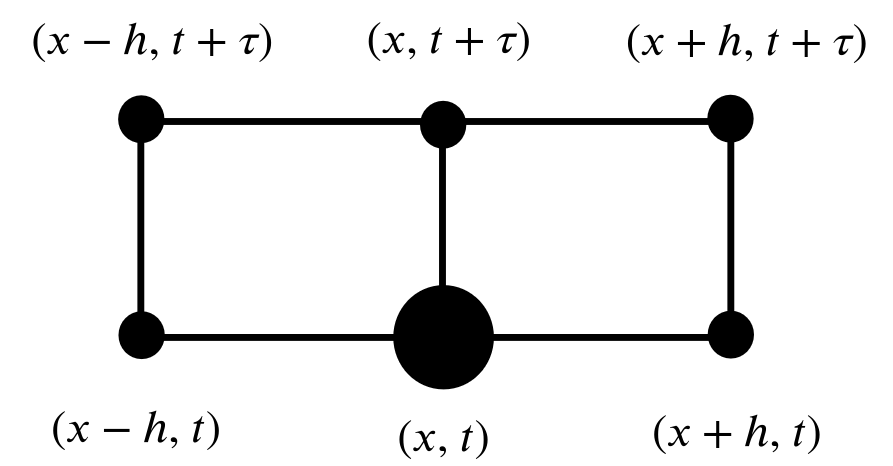
\includegraphics[scale=0.4]{images/img_5}
$$
В соответствии с методом баланса, используя данный шаблон и заменяя дифференциальные операторы разностными, можем записать разностную схему для поставленной задачи в бензиндексной форме
\begin{equation}
	\begin{cases}
		y_t = \Lambda(\sigma \hat y + (1-\sigma)y)+\varphi,\ (x,t)\in \omega_{h\tau},\\
		y(x,0) = \sin x,\ x \in \overline \omega_h,\\
		y(0,t) = \sin t,\ t \in \overline \omega_\tau,\\ 
		-y_x^{(\sigma)}(1,t) = y^{(\sigma)}(1,t) - \sqrt2\sin\left(t+1+\dfrac \pi 4\right),\ t \in \overline \omega_\tau.
	\end{cases}
\end{equation}
Здесь $$\Lambda y = (\overline a y_{\overline x})_{x},\ \hat y = y(x, t+\tau),$$
$\sigma$ -- это параметр, а из метода баланса
$$\overline a_i = \left[\dfrac 1 h \int\limits_{x_i-1}^{x_i}\dfrac{d x}{k\left(x, t_j+\dfrac \tau 2\right)}\right]^{-1},\ \text{где } k(x,t) = \cos(x+t)+1,$$
$\overline a$, $\varphi$ -- это некоторые сеточные функции. В частности, можно выбирать
$$a_i^j = k\left(x_i - \dfrac h 2, t_j + \dfrac \tau 2\right), \text{ или } a_i^j = \dfrac 12 \left[k\left(x_i - h, t_j + \dfrac \tau2\right) + k \left(x_i, t_j + \dfrac \tau2\right)\right],$$
$$\varphi_i^j = f_i^{j+\frac 12}, \text { или } \varphi_i^j = \dfrac 12(f_i^j + f_i^{j+1}).$$
\section*{Реализация разностной схемы}
Пусть $$a_i^j = k\left(x_i - \dfrac h 2, t_j + \dfrac \tau 2\right) = k_{i-\frac 12}^{j + \frac 12},\ \varphi_i^j = f_i^{j + \frac 12}$$
Алгоритм реализации будет следующий:
\begin{enumerate}
	\item нулевой слой заполняем по формуле \begin{equation}
		y_i^0 = \sin(x_i),\ i = \overline {0,N};
	\end{equation}
	\item для всех $j = \overline {0, N_1-1}$ будем вычислять $y_k^j$, решая систему линейных алгебраических уравнений с трехдиагональной матрицей, а именно
	\begin{equation}
		\begin{dcases}
			\dfrac{\sigma}{h^2}k_{i-\frac 12}^{j+\frac 12}y_{i-1}^{j+1} - \left(\dfrac{\sigma}{h^2}\left(k_{i-\frac 12}^{j + \frac 12} + k_{i + \frac 12}^{j + \frac 12}\right) + \dfrac 1 \tau\right) y_i^{j+1} + \dfrac {\sigma}{h^2}k_{i+\frac 12}^{j+\frac 12} y_{i+1}^{j+1} = - F_i^j,\ i = \overline {1, N-1},\\
			y_0^{j+1} = \sin (t_{j+1}),\\ 
			-\sigma \left(\dfrac 1 h + 1\right) y_N^{j+1} + \dfrac \sigma h y_{N-1}^{j+1} = (1-\sigma)\left(\dfrac 1 h + 1\right)y_N^j - \dfrac{(1-\sigma)}{h}y_{N-1}^j -\sqrt 2\sin\left(t_{j+1} + 1 + \dfrac \pi 4\right),
		\end{dcases}
	\end{equation}
	где $$F_k^j = \dfrac 1 \tau y_i^j + \dfrac{(1-\sigma)}{h^2}(k_{i-\frac 12}^{j+\frac 12} y_{i-1}^j - k_{i-\frac 12}^{j+\frac 12} y_i^j- k_{+\frac 12}^{j+\frac 12} y_i^j + k_{i+\frac12}^{j+\frac12}y_{i+1}^j) + f_i^{j+\frac 12}.$$
\end{enumerate}
Очевидно, что наиболее эффективным методом решения системы (15) будет метод прогонки, а сам он будет устойчивый, что следует из вида коэффициентов.

    \begin{equation}
            \begin{dcases}
                \dfrac{\sigma}{h^2}k_{i-\frac 12}^{j+\frac 12}y_{i-1}^{j+1} - \left(\dfrac{\sigma}{h^2}\left(k_{i-\frac 12}^{j + \frac 12} + k_{i + \frac 12}^{j + \frac 12}\right) + \dfrac 1 \tau\right) y_i^{j+1} + \dfrac {\sigma}{h^2}k_{i+\frac 12}^{j+\frac 12} y_{i+1}^{j+1} = - F_i^j,\ i = \overline {1, N-1},\\
                y_0^{j+1} = \cos (t_{j+1}),\\ 
                -\dfrac \sigma h y_N^{j+1} + \dfrac \sigma h y_{N-1}^{j+1} = \dfrac{(1-\sigma)}{h}(y_N^j - y_{N-1}^j) + \sin(t_{j+1} + 1),
            \end{dcases}
        \end{equation} где
\[F_k^j = \dfrac 1 \tau y_i^j + \dfrac{(1-\sigma)}{h^2}(k_{i-\frac 12}^{j+\frac 12} y_{i-1}^j - k_{i-\frac 12}^{j+\frac 12} y_i^j- k_{+\frac 12}^{j+\frac 12} y_i^j + k_{i+\frac12}^{j+\frac12}y_{i+1}^j) + f_i^{j+\frac 12}.\]

    \begin{tcolorbox}[breakable, size=fbox, boxrule=1pt, pad at break*=1mm,colback=cellbackground, colframe=cellborder]
\prompt{In}{incolor}{177}{\boxspacing}
\begin{Verbatim}[commandchars=\\\{\}]
\PY{k}{def} \PY{n+nf}{u\PYZus{}0}\PY{p}{(}\PY{n}{x}\PY{p}{)}\PY{p}{:}
    \PY{k}{return} \PY{n}{np}\PY{o}{.}\PY{n}{sin}\PY{p}{(}\PY{n}{x}\PY{p}{)}

\PY{k}{def} \PY{n+nf}{f}\PY{p}{(}\PY{n}{x}\PY{p}{,}\PY{n}{t}\PY{p}{)}\PY{p}{:}
    \PY{k}{return} \PY{p}{(}\PY{n}{x}\PY{o}{+}\PY{n}{t}\PY{o}{+}\PY{l+m+mi}{1}\PY{p}{)}\PY{o}{*}\PY{n}{np}\PY{o}{.}\PY{n}{sin}\PY{p}{(}\PY{n}{x}\PY{o}{+}\PY{n}{t}\PY{p}{)}

\PY{k}{def} \PY{n+nf}{mu\PYZus{}0}\PY{p}{(}\PY{n}{t}\PY{p}{)}\PY{p}{:}
    \PY{k}{return} \PY{n}{np}\PY{o}{.}\PY{n}{sin}\PY{p}{(}\PY{n}{t}\PY{p}{)}

\PY{k}{def} \PY{n+nf}{mu\PYZus{}1}\PY{p}{(}\PY{n}{t}\PY{p}{)}\PY{p}{:}
    \PY{k}{return} \PY{o}{\PYZhy{}}\PY{n}{np}\PY{o}{.}\PY{n}{sqrt}\PY{p}{(}\PY{l+m+mi}{2}\PY{p}{)}\PY{o}{*}\PY{n}{np}\PY{o}{.}\PY{n}{sin}\PY{p}{(}\PY{n}{t} \PY{o}{+} \PY{l+m+mi}{1} \PY{o}{+} \PY{n}{np}\PY{o}{.}\PY{n}{pi}\PY{o}{/}\PY{l+m+mi}{4}\PY{p}{)}

\PY{k}{def} \PY{n+nf}{k}\PY{p}{(}\PY{n}{x}\PY{p}{,}\PY{n}{t}\PY{p}{)}\PY{p}{:}
    \PY{k}{return} \PY{n}{x} \PY{o}{+} \PY{n}{t} \PY{o}{+} \PY{l+m+mi}{1}
\end{Verbatim}
\end{tcolorbox}

    \begin{tcolorbox}[breakable, size=fbox, boxrule=1pt, pad at break*=1mm,colback=cellbackground, colframe=cellborder]
\prompt{In}{incolor}{178}{\boxspacing}
\begin{Verbatim}[commandchars=\\\{\}]
\PY{k}{def} \PY{n+nf}{diff\PYZus{}scheme\PYZus{}solve}\PY{p}{(}\PY{n}{x}\PY{p}{,} \PY{n}{t}\PY{p}{,} \PY{n}{h}\PY{p}{,} \PY{n}{tau}\PY{p}{,} \PY{n}{sigma}\PY{p}{,} \PY{n}{f}\PY{p}{,} \PY{n}{u\PYZus{}0}\PY{p}{,} \PY{n}{mu\PYZus{}0}\PY{p}{,} \PY{n}{mu\PYZus{}1}\PY{p}{,} \PY{n}{k}\PY{p}{)}\PY{p}{:}

    \PY{n}{y} \PY{o}{=} \PY{n}{np}\PY{o}{.}\PY{n}{zeros}\PY{p}{(}\PY{p}{(}\PY{n+nb}{len}\PY{p}{(}\PY{n}{x}\PY{p}{)}\PY{p}{,} \PY{n+nb}{len}\PY{p}{(}\PY{n}{t}\PY{p}{)}\PY{p}{)}\PY{p}{)}

    \PY{k}{for} \PY{n}{i} \PY{o+ow}{in} \PY{n+nb}{range}\PY{p}{(}\PY{n+nb}{len}\PY{p}{(}\PY{n}{x}\PY{p}{)}\PY{p}{)}\PY{p}{:}
        \PY{n}{y}\PY{p}{[}\PY{n}{i}\PY{p}{,} \PY{l+m+mi}{0}\PY{p}{]} \PY{o}{=} \PY{n}{u\PYZus{}0}\PY{p}{(}\PY{n}{x}\PY{p}{[}\PY{n}{i}\PY{p}{]}\PY{p}{)}

    \PY{k}{for} \PY{n}{j} \PY{o+ow}{in} \PY{n+nb}{range}\PY{p}{(}\PY{n+nb}{len}\PY{p}{(}\PY{n}{t}\PY{p}{)}\PY{o}{\PYZhy{}}\PY{l+m+mi}{1}\PY{p}{)}\PY{p}{:}
        \PY{n}{gamma} \PY{o}{=} \PY{p}{[}\PY{l+m+mi}{1}\PY{p}{]}
        \PY{n}{beta} \PY{o}{=} \PY{p}{[}\PY{l+m+mi}{0}\PY{p}{]}
        \PY{n}{g} \PY{o}{=} \PY{p}{[}\PY{n}{mu\PYZus{}0}\PY{p}{(}\PY{n}{t}\PY{p}{[}\PY{n}{j}\PY{o}{+}\PY{l+m+mi}{1}\PY{p}{]}\PY{p}{)}\PY{p}{]} 
        \PY{n}{alpha} \PY{o}{=} \PY{p}{[}\PY{l+m+mi}{0}\PY{p}{]}
        \PY{k}{for} \PY{n}{i} \PY{o+ow}{in} \PY{n+nb}{range}\PY{p}{(}\PY{l+m+mi}{1}\PY{p}{,} \PY{n+nb}{len}\PY{p}{(}\PY{n}{x}\PY{p}{)}\PY{o}{\PYZhy{}}\PY{l+m+mi}{1}\PY{p}{)}\PY{p}{:}
            \PY{n}{alpha}\PY{o}{.}\PY{n}{append}\PY{p}{(}\PY{n}{sigma}\PY{o}{/}\PY{n}{h}\PY{o}{*}\PY{o}{*}\PY{l+m+mi}{2} \PY{o}{*} \PY{n}{k}\PY{p}{(}\PY{n}{x}\PY{p}{[}\PY{n}{i}\PY{p}{]} \PY{o}{\PYZhy{}} \PY{n}{h}\PY{o}{/}\PY{l+m+mi}{2}\PY{p}{,} \PY{n}{t}\PY{p}{[}\PY{n}{j}\PY{p}{]} \PY{o}{+} \PY{n}{tau}\PY{o}{/}\PY{l+m+mi}{2}\PY{p}{)}\PY{p}{)}
            \PY{n}{gamma}\PY{o}{.}\PY{n}{append}\PY{p}{(}\PY{o}{\PYZhy{}}\PY{p}{(}\PY{n}{sigma} \PY{o}{/} \PY{n}{h}\PY{o}{*}\PY{o}{*}\PY{l+m+mi}{2}\PY{o}{*}\PY{p}{(}\PY{n}{k}\PY{p}{(}\PY{n}{x}\PY{p}{[}\PY{n}{i}\PY{p}{]} \PY{o}{\PYZhy{}} \PY{n}{h}\PY{o}{/}\PY{l+m+mi}{2}\PY{p}{,} \PY{n}{t}\PY{p}{[}\PY{n}{j}\PY{p}{]} \PY{o}{+} \PY{n}{tau}\PY{o}{/}\PY{l+m+mi}{2}\PY{p}{)} \PY{o}{+} \PY{n}{k}\PY{p}{(}\PY{n}{x}\PY{p}{[}\PY{n}{i}\PY{p}{]} \PY{o}{+} \PY{n}{h}\PY{o}{/}\PY{l+m+mi}{2}\PY{p}{,} \PY{n}{t}\PY{p}{[}\PY{n}{j}\PY{p}{]} \PY{o}{+} \PY{n}{tau}\PY{o}{/}\PY{l+m+mi}{2}\PY{p}{)}\PY{p}{)}\PY{o}{+}\PY{l+m+mi}{1}\PY{o}{/}\PY{n}{tau}\PY{p}{)}\PY{p}{)}
            \PY{n}{beta}\PY{o}{.}\PY{n}{append}\PY{p}{(}\PY{n}{sigma}\PY{o}{/}\PY{n}{h}\PY{o}{*}\PY{o}{*}\PY{l+m+mi}{2}\PY{o}{*}\PY{n}{k}\PY{p}{(}\PY{n}{x}\PY{p}{[}\PY{n}{i}\PY{p}{]} \PY{o}{+} \PY{n}{h}\PY{o}{/}\PY{l+m+mi}{2}\PY{p}{,} \PY{n}{t}\PY{p}{[}\PY{n}{j}\PY{p}{]} \PY{o}{+} \PY{n}{tau}\PY{o}{/}\PY{l+m+mi}{2}\PY{p}{)}\PY{p}{)}
            \PY{n}{g}\PY{o}{.}\PY{n}{append}\PY{p}{(}\PY{o}{\PYZhy{}}\PY{p}{(}\PY{l+m+mi}{1}\PY{o}{/}\PY{n}{tau}\PY{o}{*}\PY{n}{y}\PY{p}{[}\PY{n}{i}\PY{p}{,}\PY{n}{j}\PY{p}{]} \PY{o}{+} \PY{p}{(}\PY{l+m+mi}{1}\PY{o}{\PYZhy{}}\PY{n}{sigma}\PY{p}{)}\PY{o}{*}\PY{p}{(}\PY{n}{k}\PY{p}{(}\PY{n}{x}\PY{p}{[}\PY{n}{i}\PY{p}{]} \PY{o}{\PYZhy{}} \PY{n}{h}\PY{o}{/}\PY{l+m+mi}{2}\PY{p}{,} \PY{n}{t}\PY{p}{[}\PY{n}{j}\PY{p}{]} \PY{o}{+} \PY{n}{tau}\PY{o}{/}\PY{l+m+mi}{2}\PY{p}{)}\PY{o}{*}\PY{n}{y}\PY{p}{[}\PY{n}{i}\PY{o}{\PYZhy{}}\PY{l+m+mi}{1}\PY{p}{,} \PY{n}{j}\PY{p}{]} \PY{o}{\PYZhy{}} \PY{n}{k}\PY{p}{(}\PY{n}{x}\PY{p}{[}\PY{n}{i}\PY{p}{]} \PY{o}{\PYZhy{}} \PY{n}{h}\PY{o}{/}\PY{l+m+mi}{2}\PY{p}{,} \PY{n}{t}\PY{p}{[}\PY{n}{j}\PY{p}{]} \PY{o}{+} \PY{n}{tau}\PY{o}{/}\PY{l+m+mi}{2}\PY{p}{)}\PY{o}{*}\PY{n}{y}\PY{p}{[}\PY{n}{i}\PY{p}{,}\PY{n}{j}\PY{p}{]} \PY{o}{\PYZhy{}} \PY{n}{k}\PY{p}{(}\PY{n}{x}\PY{p}{[}\PY{n}{i}\PY{p}{]} \PY{o}{+} \PY{n}{h}\PY{o}{/}\PY{l+m+mi}{2}\PY{p}{,} \PY{n}{t}\PY{p}{[}\PY{n}{j}\PY{p}{]} \PY{o}{+} \PY{n}{tau}\PY{o}{/}\PY{l+m+mi}{2}\PY{p}{)}\PY{o}{*}\PY{n}{y}\PY{p}{[}\PY{n}{i}\PY{p}{,}\PY{n}{j}\PY{p}{]} \PY{o}{+} \PY{n}{k}\PY{p}{(}\PY{n}{x}\PY{p}{[}\PY{n}{i}\PY{p}{]} \PY{o}{+} \PY{n}{h}\PY{o}{/}\PY{l+m+mi}{2}\PY{p}{,} \PY{n}{t}\PY{p}{[}\PY{n}{j}\PY{p}{]} \PY{o}{+} \PY{n}{tau}\PY{o}{/}\PY{l+m+mi}{2}\PY{p}{)}\PY{o}{*}\PY{n}{y}\PY{p}{[}\PY{n}{i}\PY{o}{+}\PY{l+m+mi}{1}\PY{p}{,}\PY{n}{j}\PY{p}{]}\PY{p}{)}\PY{o}{/}\PY{n}{h}\PY{o}{*}\PY{o}{*}\PY{l+m+mi}{2} \PY{o}{+} \PY{n}{f}\PY{p}{(}\PY{n}{x}\PY{p}{[}\PY{n}{i}\PY{p}{]}\PY{p}{,} \PY{n}{t}\PY{p}{[}\PY{n}{j}\PY{p}{]}\PY{o}{+}\PY{n}{tau}\PY{o}{/}\PY{l+m+mi}{2}\PY{p}{)}\PY{p}{)}\PY{p}{)}
        \PY{n}{alpha}\PY{o}{.}\PY{n}{append}\PY{p}{(}\PY{n}{sigma}\PY{o}{/}\PY{n}{h}\PY{p}{)}
        \PY{n}{gamma}\PY{o}{.}\PY{n}{append}\PY{p}{(}\PY{o}{\PYZhy{}}\PY{n}{sigma}\PY{o}{*}\PY{p}{(}\PY{l+m+mi}{1}\PY{o}{/}\PY{n}{h}\PY{o}{+}\PY{l+m+mi}{1}\PY{p}{)}\PY{p}{)}
        \PY{n}{g}\PY{o}{.}\PY{n}{append}\PY{p}{(}\PY{p}{(}\PY{l+m+mi}{1}\PY{o}{\PYZhy{}}\PY{n}{sigma}\PY{p}{)}\PY{o}{*}\PY{p}{(}\PY{l+m+mi}{1}\PY{o}{/}\PY{n}{h}\PY{o}{+}\PY{l+m+mi}{1}\PY{p}{)}\PY{o}{*}\PY{n}{y}\PY{p}{[}\PY{n+nb}{len}\PY{p}{(}\PY{n}{x}\PY{p}{)}\PY{o}{\PYZhy{}}\PY{l+m+mi}{1}\PY{p}{,} \PY{n}{j}\PY{p}{]} \PY{o}{\PYZhy{}} \PY{p}{(}\PY{l+m+mi}{1}\PY{o}{\PYZhy{}}\PY{n}{sigma}\PY{p}{)}\PY{o}{/}\PY{n}{h}\PY{o}{*}\PY{n}{y}\PY{p}{[}\PY{n+nb}{len}\PY{p}{(}\PY{n}{x}\PY{p}{)}\PY{o}{\PYZhy{}}\PY{l+m+mi}{2}\PY{p}{,}\PY{n}{j}\PY{p}{]} \PY{o}{+} \PY{n}{mu\PYZus{}1}\PY{p}{(}\PY{n}{t}\PY{p}{[}\PY{n}{j}\PY{o}{+}\PY{l+m+mi}{1}\PY{p}{]}\PY{p}{)}\PY{p}{)}
        \PY{n}{beta}\PY{o}{.}\PY{n}{append}\PY{p}{(}\PY{l+m+mi}{0}\PY{p}{)}
        \PY{n}{y}\PY{p}{[}\PY{p}{:}\PY{p}{,} \PY{n}{j}\PY{o}{+}\PY{l+m+mi}{1}\PY{p}{]} \PY{o}{=} \PY{n}{tridiagonal\PYZus{}algorithm}\PY{p}{(}\PY{n}{alpha}\PY{p}{,}\PY{n}{beta}\PY{p}{,}\PY{n}{gamma}\PY{p}{,}\PY{n}{g}\PY{p}{)}

    \PY{k}{return} \PY{n}{y}
\end{Verbatim}
\end{tcolorbox}

    \begin{tcolorbox}[breakable, size=fbox, boxrule=1pt, pad at break*=1mm,colback=cellbackground, colframe=cellborder]
\prompt{In}{incolor}{180}{\boxspacing}
\begin{Verbatim}[commandchars=\\\{\}]
\PY{n}{h}\PY{p}{,} \PY{n}{x\PYZus{}grid} \PY{o}{=} \PY{n}{generate\PYZus{}grid}\PY{p}{(}\PY{l+m+mi}{1}\PY{p}{,} \PY{l+m+mi}{100}\PY{p}{)}
\PY{n}{tau}\PY{p}{,} \PY{n}{t\PYZus{}grid} \PY{o}{=} \PY{n}{generate\PYZus{}grid}\PY{p}{(}\PY{l+m+mi}{10}\PY{p}{,} \PY{l+m+mi}{100}\PY{p}{)}
\end{Verbatim}
\end{tcolorbox}

    \begin{tcolorbox}[breakable, size=fbox, boxrule=1pt, pad at break*=1mm,colback=cellbackground, colframe=cellborder]
\prompt{In}{incolor}{181}{\boxspacing}
\begin{Verbatim}[commandchars=\\\{\}]
\PY{n+nb}{print}\PY{p}{(}\PY{l+s+s1}{\PYZsq{}}\PY{l+s+s1}{tau=}\PY{l+s+s1}{\PYZsq{}} \PY{o}{+} \PY{n+nb}{str}\PY{p}{(}\PY{n}{tau}\PY{p}{)} \PY{o}{+} \PY{l+s+s1}{\PYZsq{}}\PY{l+s+se}{\PYZbs{}n}\PY{l+s+s1}{h=}\PY{l+s+s1}{\PYZsq{}} \PY{o}{+} \PY{n+nb}{str}\PY{p}{(}\PY{n}{h}\PY{p}{)}\PY{p}{)} 
\end{Verbatim}
\end{tcolorbox}

    \begin{Verbatim}[commandchars=\\\{\}]
tau=0.1
h=0.01
    \end{Verbatim}

    \begin{tcolorbox}[breakable, size=fbox, boxrule=1pt, pad at break*=1mm,colback=cellbackground, colframe=cellborder]
\prompt{In}{incolor}{187}{\boxspacing}
\begin{Verbatim}[commandchars=\\\{\}]
\PY{n}{sigma} \PY{o}{=} \PY{l+m+mi}{1}\PY{o}{/}\PY{l+m+mi}{2}
\end{Verbatim}
\end{tcolorbox}

    Находим приближенное решение

    \begin{tcolorbox}[breakable, size=fbox, boxrule=1pt, pad at break*=1mm,colback=cellbackground, colframe=cellborder]
\prompt{In}{incolor}{188}{\boxspacing}
\begin{Verbatim}[commandchars=\\\{\}]
\PY{n}{y} \PY{o}{=} \PY{n}{diff\PYZus{}scheme\PYZus{}solve}\PY{p}{(}\PY{n}{x\PYZus{}grid}\PY{p}{,} \PY{n}{t\PYZus{}grid}\PY{p}{,} \PY{n}{h}\PY{p}{,} \PY{n}{tau}\PY{p}{,} \PY{n}{sigma}\PY{p}{,} \PY{n}{f}\PY{p}{,} \PY{n}{u\PYZus{}0}\PY{p}{,} \PY{n}{mu\PYZus{}0}\PY{p}{,} \PY{n}{mu\PYZus{}1}\PY{p}{,} \PY{n}{k}\PY{p}{)}
\end{Verbatim}
\end{tcolorbox}

    \begin{tcolorbox}[breakable, size=fbox, boxrule=1pt, pad at break*=1mm,colback=cellbackground, colframe=cellborder]
\prompt{In}{incolor}{189}{\boxspacing}
\begin{Verbatim}[commandchars=\\\{\}]
\PY{n}{print\PYZus{}exact}\PY{p}{(}\PY{p}{)}
\PY{n}{print\PYZus{}approx}\PY{p}{(}\PY{p}{)}
\end{Verbatim}
\end{tcolorbox}

    \begin{center}
    \adjustimage{max size={0.9\linewidth}{0.9\paperheight}}{output_33_0.png}
    \end{center}
    { \hspace*{\fill} \\}
    
    \begin{center}
    \adjustimage{max size={0.9\linewidth}{0.9\paperheight}}{output_33_1.png}
    \end{center}
    { \hspace*{\fill} \\}
    

    % Add a bibliography block to the postdoc
    
    
    
\end{document}
